\documentclass[11pt, french]{beamer}

\usepackage[utf8]{inputenc}
\usepackage[T1]{fontenc}
\usepackage[french]{babel}
\usepackage{graphicx}
\usepackage{xcolor}
\usepackage{tikz}

% ─── Thème et couleurs ────────────────────────────────────────────────
\usetheme{Madrid}
\usecolortheme{default}

% Couleurs personnalisées
\definecolor{darkblue}{rgb}{0.1, 0.3, 0.5}
\definecolor{lightblue}{rgb}{0.2, 0.4, 0.7}
\definecolor{accentred}{rgb}{1, 0.3, 0.2}

\setbeamercolor{palette primary}{bg=darkblue, fg=white}
\setbeamercolor{palette secondary}{bg=lightblue, fg=white}
\setbeamercolor{palette tertiary}{bg=accentred, fg=white}
\setbeamercolor{title}{fg=darkblue}
\setbeamercolor{subtitle}{fg=lightblue}

% ─── En-têtes et pieds de page ────────────────────────────────────────
\setbeamerfont{page number in head/foot}{size=\small}
\setbeamertemplate{footline}[frame number]

% ─── Commandes personnalisées ─────────────────────────────────────────
\newcommand{\todo}[1]{{\color{red}\textbf{[À MODIFIER: #1]}}}
\newcommand{\placeholder}[2]{
  \begin{center}
  \fbox{\begin{minipage}{#1}
    \centering
    \textit{\small Image / Schéma : #2}
    \vspace{#1}
  \end{minipage}}
  \end{center}
}

% ─── Titres et auteur ─────────────────────────────────────────────────
\title{Pepper Battleship}
\subtitle{Étude de la confiance accordée à un humain vs une IA}
\author{\todo{Prénom NOM}, \todo{Prénom NOM}}
\date{\today}
\institute{Master 1 Génie Logiciel \\ Faculté des Sciences -- Département Informatique}

% ═════════════════════════════════════════════════════════════════════════
% DÉBUT DU DOCUMENT
% ═════════════════════════════════════════════════════════════════════════

\begin{document}

% ─── Diapo de titre ───────────────────────────────────────────────────
\begin{frame}
\maketitle
\end{frame}

% ─── Plan ─────────────────────────────────────────────────────────────
\begin{frame}
\frametitle{Plan}
\tableofcontents
\end{frame}

% ═════════════════════════════════════════════════════════════════════════
% SECTION 1 : INTRODUCTION
% ═════════════════════════════════════════════════════════════════════════

\section{Introduction}

\begin{frame}
\frametitle{Motivation}
\begin{itemize}
    \item \textbf{Question fondamentale} : Les utilisateurs accordent-ils différemment leur confiance à un adversaire humain vs une IA ?
    \vspace{0.5cm}
    \item \textbf{Contexte} : Omniprésence de l'IA dans les interactions quotidiennes
    \vspace{0.5cm}
    \item \textbf{Enjeu} : Conception d'interfaces homme-machine éthiques et fiables
\end{itemize}
\end{frame}

\begin{frame}
\frametitle{État de l'art}
\begin{columns}[T]
\column{0.5\textwidth}
\textbf{Théorie de l'attribution}
\begin{itemize}
    \item Heider (1958), Weiner (1985)
    \item Explications causales biaisées pour les machines
\end{itemize}

\column{0.5\textwidth}
\textbf{Étude Ullman et al. (2014)}
\begin{itemize}
    \item Yale University
    \item Confiance vs tromperie du robot
\end{itemize}
\end{columns}

\vspace{1cm}

\textbf{Anthropomorphisme inversé}
\begin{itemize}
    \item Standards moraux différents selon la cible
    \item Machines jugées plus sévèrement
\end{itemize}
\end{frame}

\begin{frame}
\frametitle{Hypothèses de recherche}
\begin{enumerate}
    \item[\textbf{H\textsubscript{1}}] Les participants expriment une évaluation de déloyauté \textbf{significativement plus élevée} pour le CheatBot que pour le même comportement attribué à un humain
    
    \vspace{0.5cm}
    
    \item[\textbf{H\textsubscript{2a}}] L'écart de confiance \textbf{diminue} au fil des tours (apprentissage)
    
    \vspace{0.5cm}
    
    \item[\textbf{H\textsubscript{2b}}] L'ordre de présentation \textbf{influence} les perceptions ultérieures
\end{enumerate}
\end{frame}

% ═════════════════════════════════════════════════════════════════════════
% SECTION 2 : CONTEXTE DU PROJET
% ═════════════════════════════════════════════════════════════════════════

\section{Contexte du Projet}

\begin{frame}
\frametitle{De Pepper à la plateforme digitale}
\begin{columns}[T]
\column{0.5\textwidth}
\textbf{Phase 1 : Robot Pepper}
\begin{itemize}
    \item Objectif initial : humain vs humanoïde vs digital
    \item Intégration avec robot social SoftBank
\end{itemize}

\column{0.5\textwidth}
\textbf{Problèmes rencontrés}
\begin{itemize}
    \item Parties trop longues (15-30s latence)
    \item Confonds expérimentaux
    \item Expérience frustrante
\end{itemize}
\end{columns}

\vspace{1cm}
\hrule
\vspace{1cm}

\textbf{Phase 2 : Pivot vers digital}
\begin{itemize}
    \item Maintien de Python (infrastructure Pepper déjà développée)
    \item Ajout de couche web (Flask)
    \item Avantage : contrôle rigoureux, reproductibilité, scalabilité
\end{itemize}
\end{frame}

% ═════════════════════════════════════════════════════════════════════════
% SECTION 3 : DÉVELOPPEMENT (SECTION PRINCIPALE)
% ═════════════════════════════════════════════════════════════════════════

\section{Développement}

\subsection{Architecture générale}

\begin{frame}
\frametitle{Architecture générale}
\begin{center}
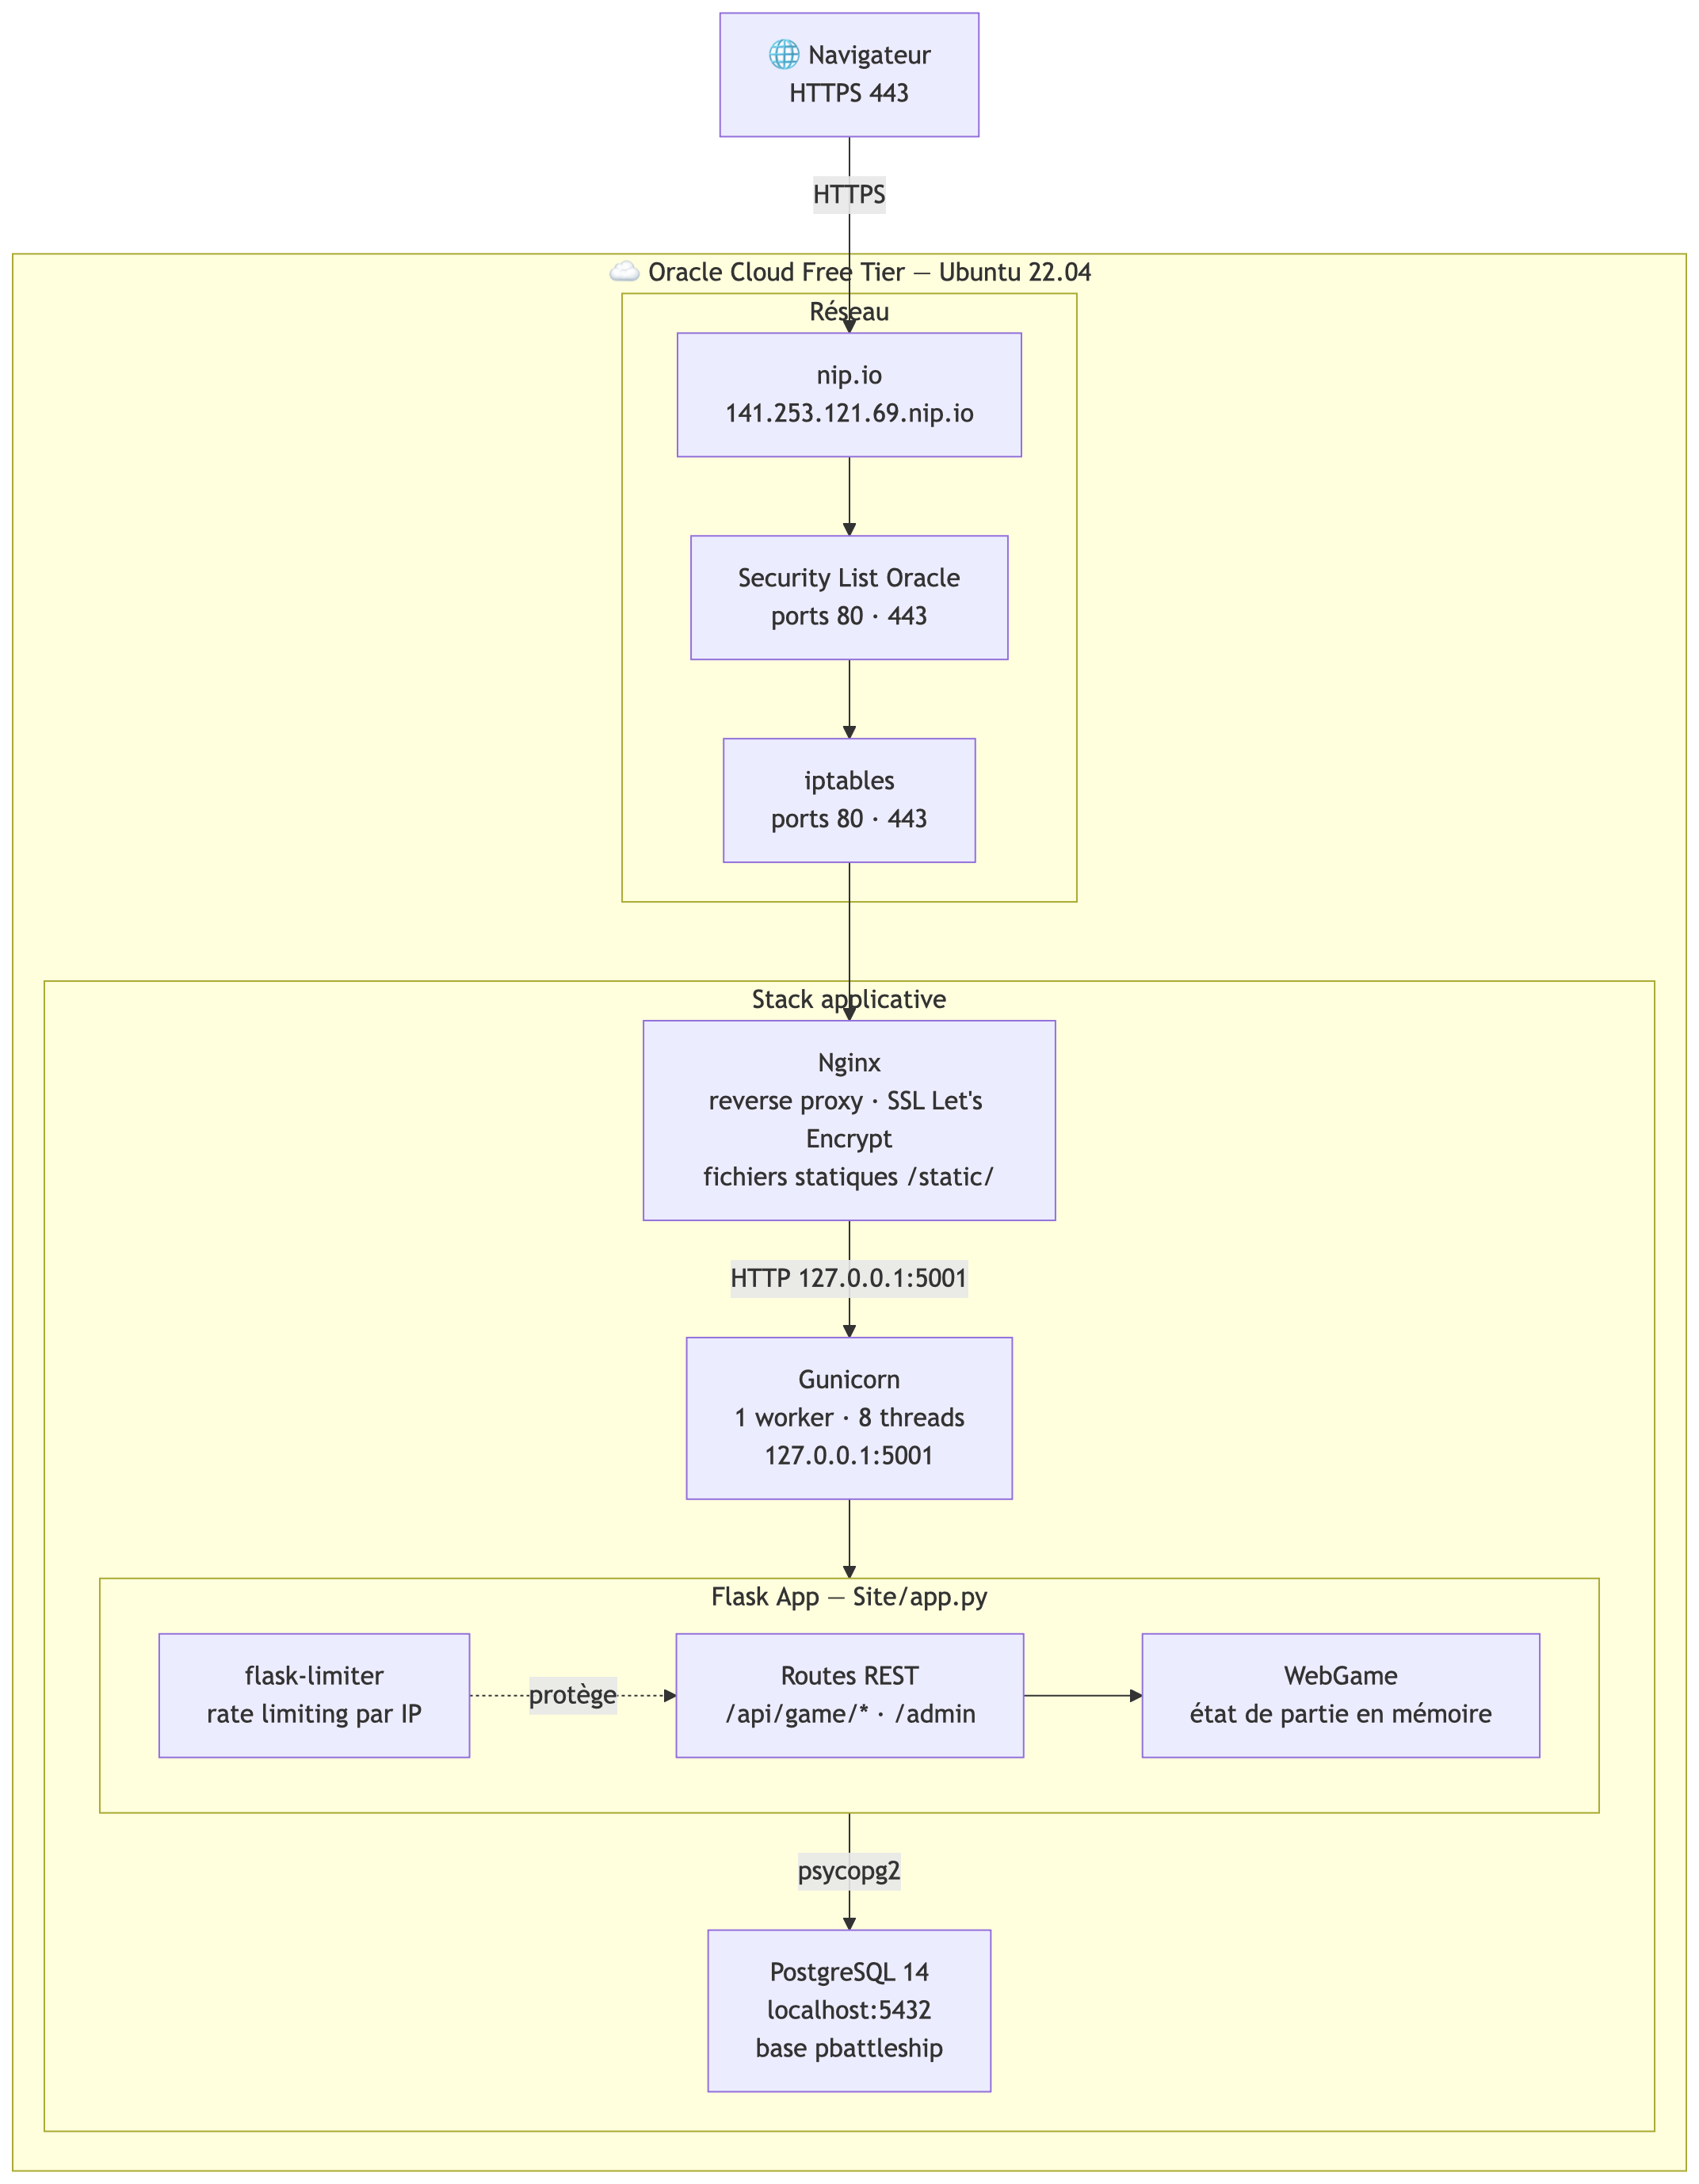
\includegraphics[width=0.85\textwidth]{../rapport/diagrams/images/architecture_globale.png}
\end{center}

\vspace{0.5cm}

\textbf{Composants clés :}
\begin{itemize}
    \item \textbf{Backend Python} : Logique métier, CheatBot, gestion de base de données
    \item \textbf{Frontend Web} : Interface utilisateur (Flask + JavaScript)
    \item \textbf{Communication} : API REST
\end{itemize}
\end{frame}

\begin{frame}
\frametitle{Stack technologique}
\begin{columns}[T]
\column{0.33\textwidth}
\textbf{Backend Python}
\begin{itemize}
    \item Python 3.x
    \item Architecture modulaire
    \item SQLite
    \item Socket TCP/IP
\end{itemize}

\column{0.33\textwidth}
\textbf{Frontend Web}
\begin{itemize}
    \item Flask 2.3+
    \item API REST
    \item HTML5 + CSS3
    \item JavaScript vanilla
\end{itemize}

\column{0.33\textwidth}
\textbf{Communication}
\begin{itemize}
    \item API REST JSON
    \item Session management
    \item Base SQLite centralisée
\end{itemize}
\end{columns}
\end{frame}

\subsection{Plateforme Web}

\begin{frame}
\frametitle{Plateforme Web : Vue d'ensemble}
\begin{center}
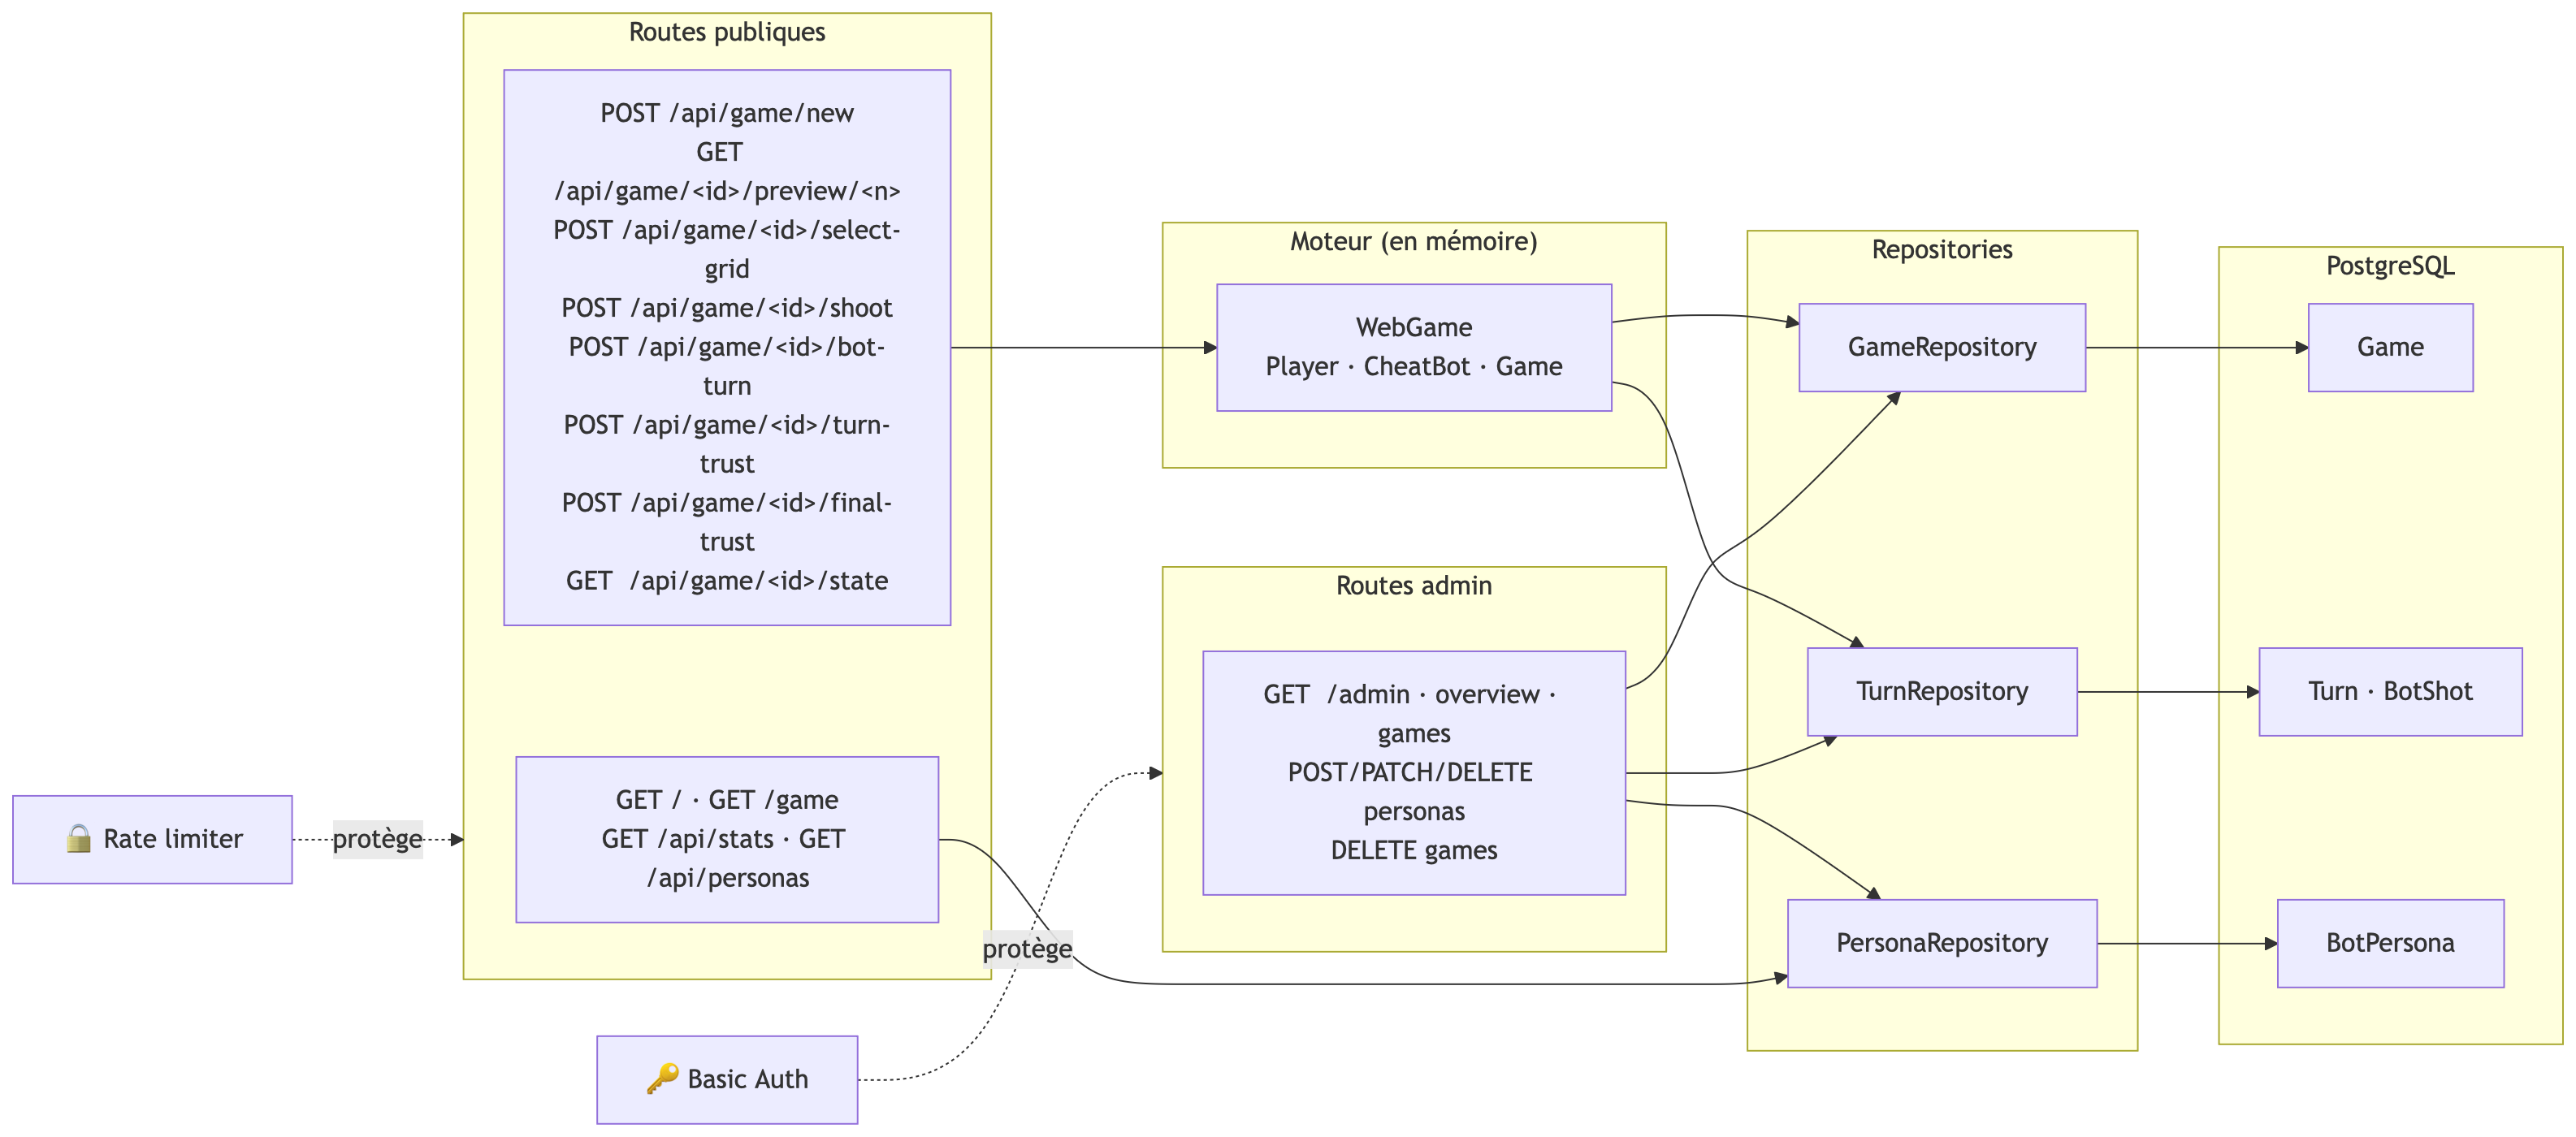
\includegraphics[width=0.90\textwidth]{../rapport/diagrams/images/backend.png}
\end{center}
\end{frame}

\begin{frame}
\frametitle{Landing Page (index.html)}
\begin{columns}[T]
\column{0.5\textwidth}
\textbf{Sections principales :}
\begin{enumerate}
    \item Navigation
    \item Héros (appel à l'action)
    \item 6 cartes de fonctionnalités
    \item Tutoriel (4 étapes)
    \item Section recherche
\end{enumerate}

\column{0.5\textwidth}
\begin{center}
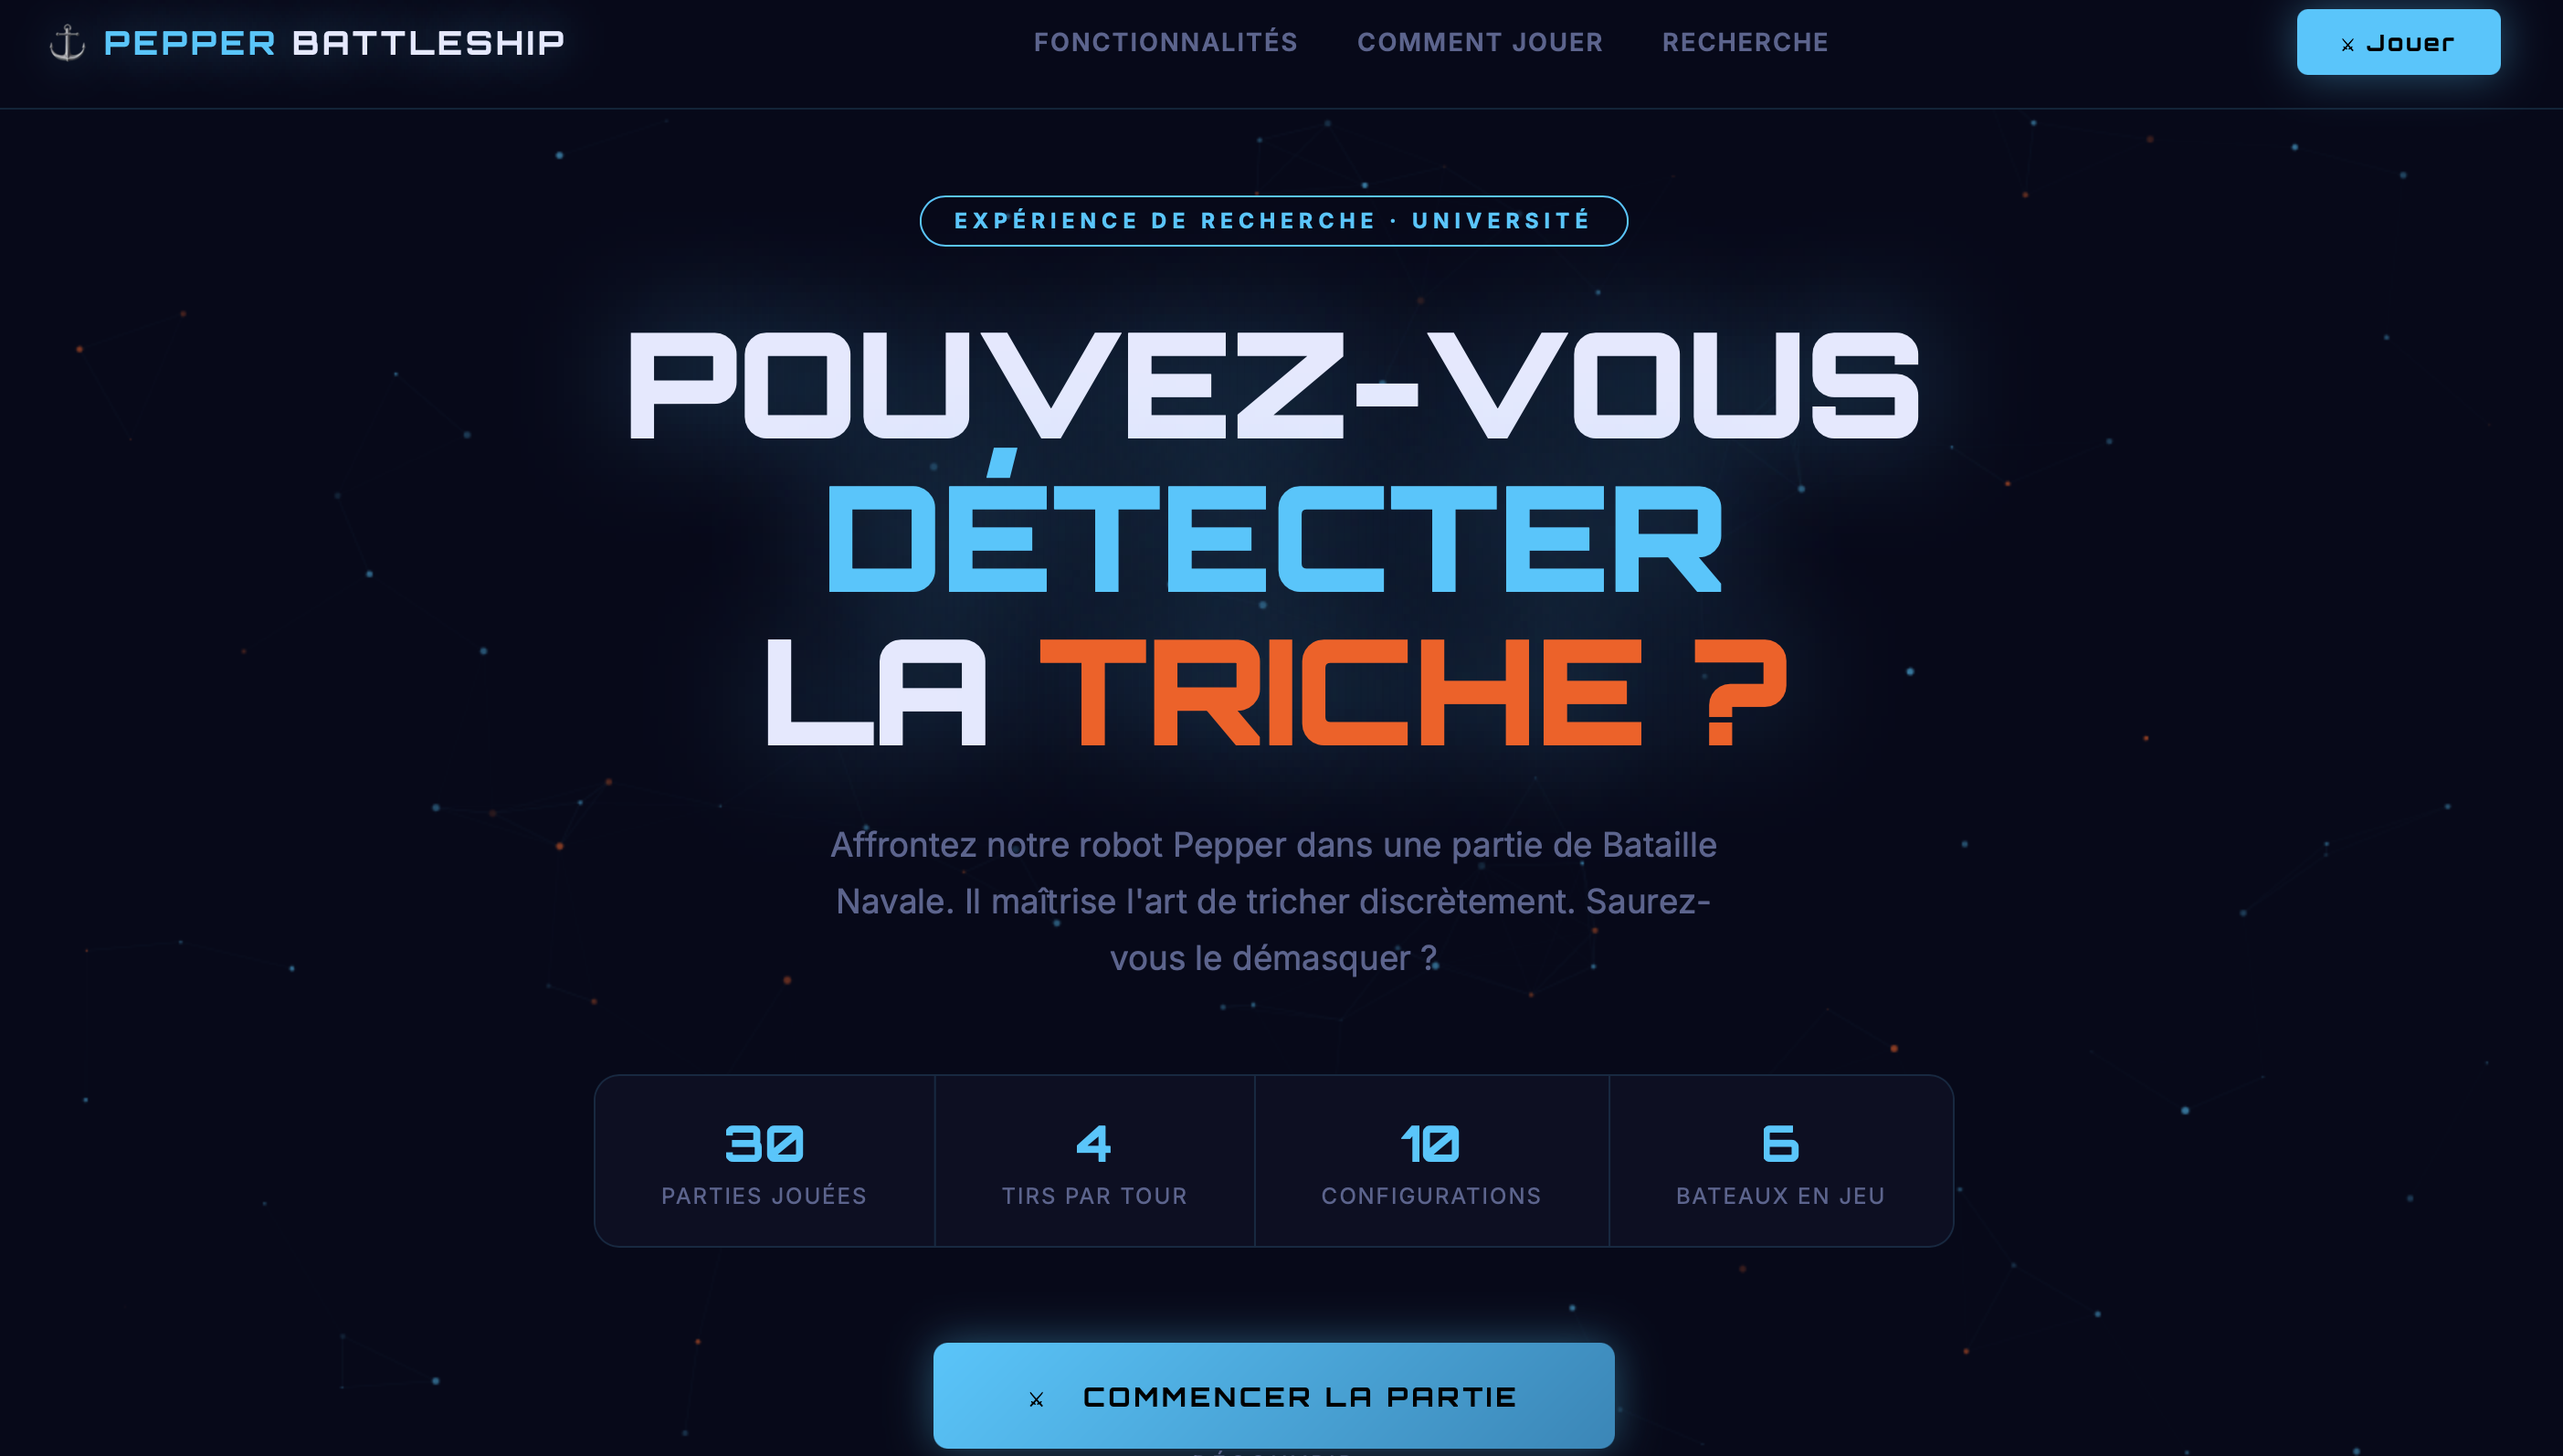
\includegraphics[width=0.45\textwidth]{../rapport/diagrams/interfaces_site/accueil.png}
\end{center}
\end{columns}
\end{frame}

\begin{frame}
\frametitle{Interface de Jeu Web}
\textbf{Machine à états (5 phases) :}
\begin{enumerate}
    \item \textbf{Setup} : Entrée du nom du joueur
    \item \textbf{Persona} : Sélection du contexte (humain vs robot)
    \item \textbf{Grid} : Validation configuration de flotte
    \item \textbf{Playing} : Jeu et collecte de scores de confiance
    \item \textbf{GameOver} : Résultats et débriefing
\end{enumerate}

\vspace{0.5cm}
\begin{center}
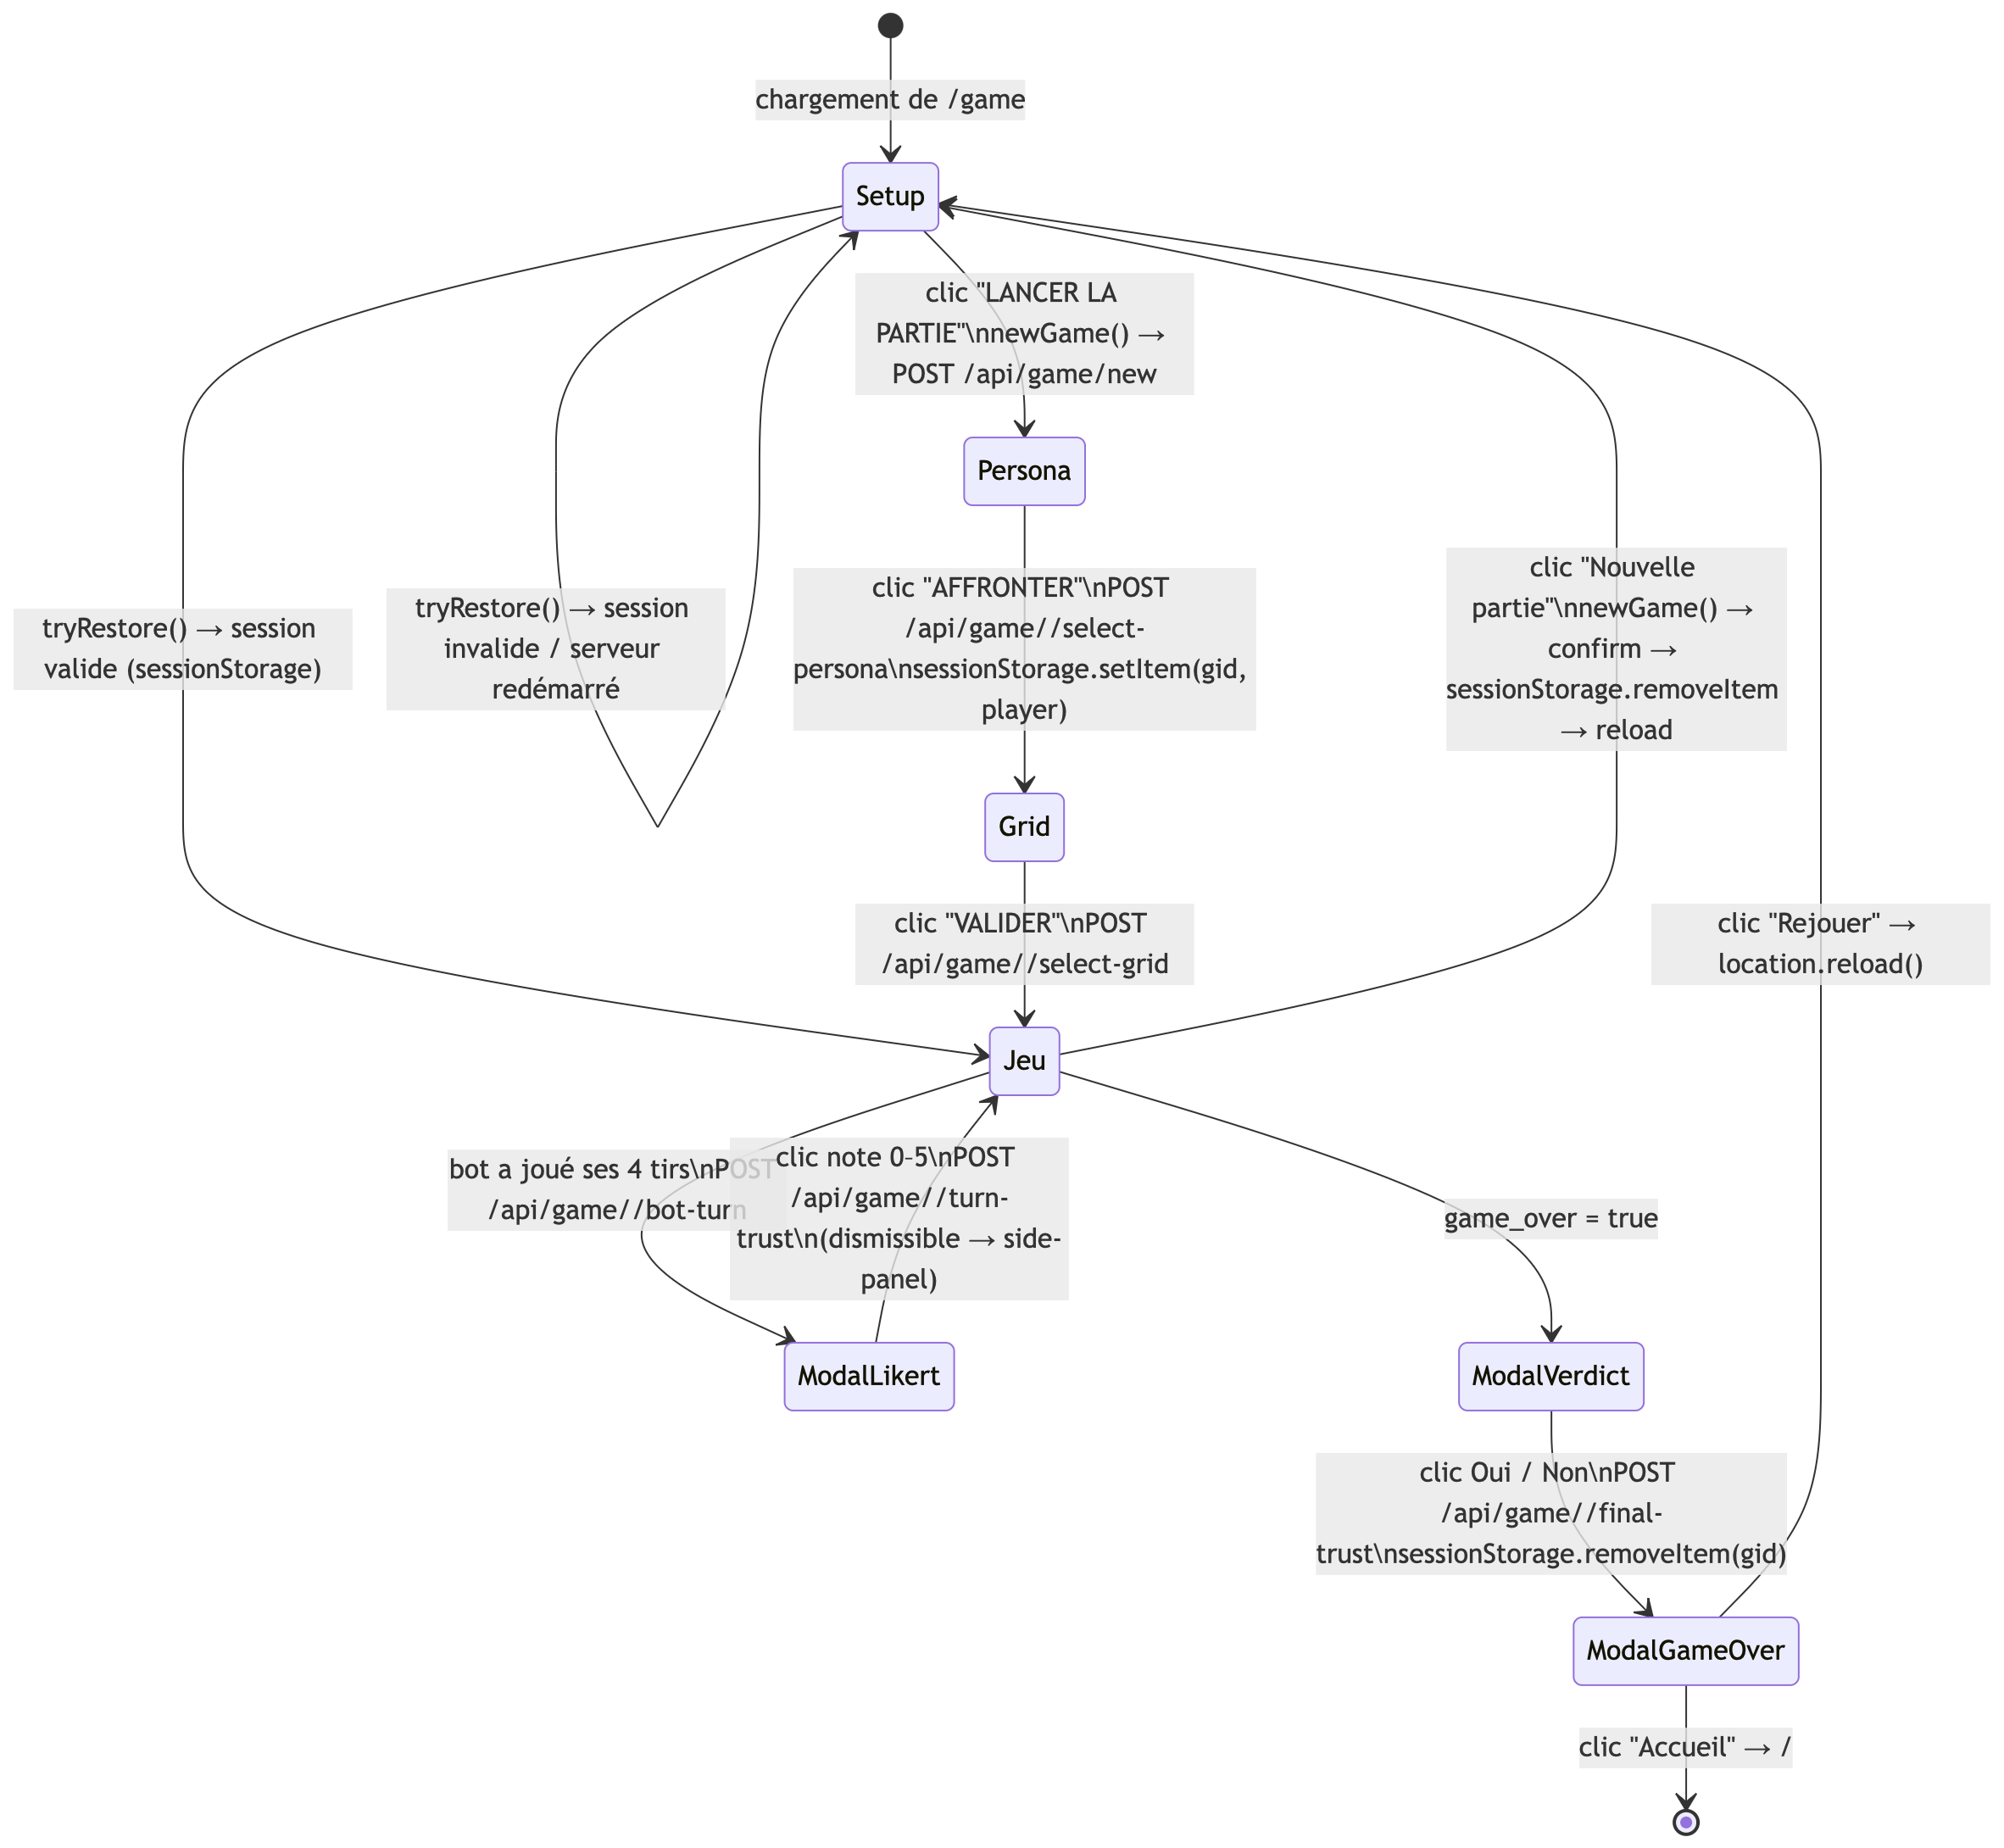
\includegraphics[width=0.70\textwidth]{../rapport/diagrams/images/Front/MachineEtat_Ecran.png}
\end{center}
\end{frame}

\begin{frame}
\frametitle{Grilles de jeu (10×10)}
\begin{columns}[T]
\column{0.5\textwidth}
\textbf{Grille du joueur :}
\begin{itemize}
    \item Ma flotte (6 bateaux)
    \item Tirs ennemis reçus
    \item Symboles : ~ X C *
\end{itemize}

\column{0.5\textwidth}
\textbf{Grille de suivi :}
\begin{itemize}
    \item Mes tirs effectués
    \item Résultats (touché/raté/coulé)
    \item Visualisation en temps réel
\end{itemize}
\end{columns}

\vspace{1cm}
\begin{center}
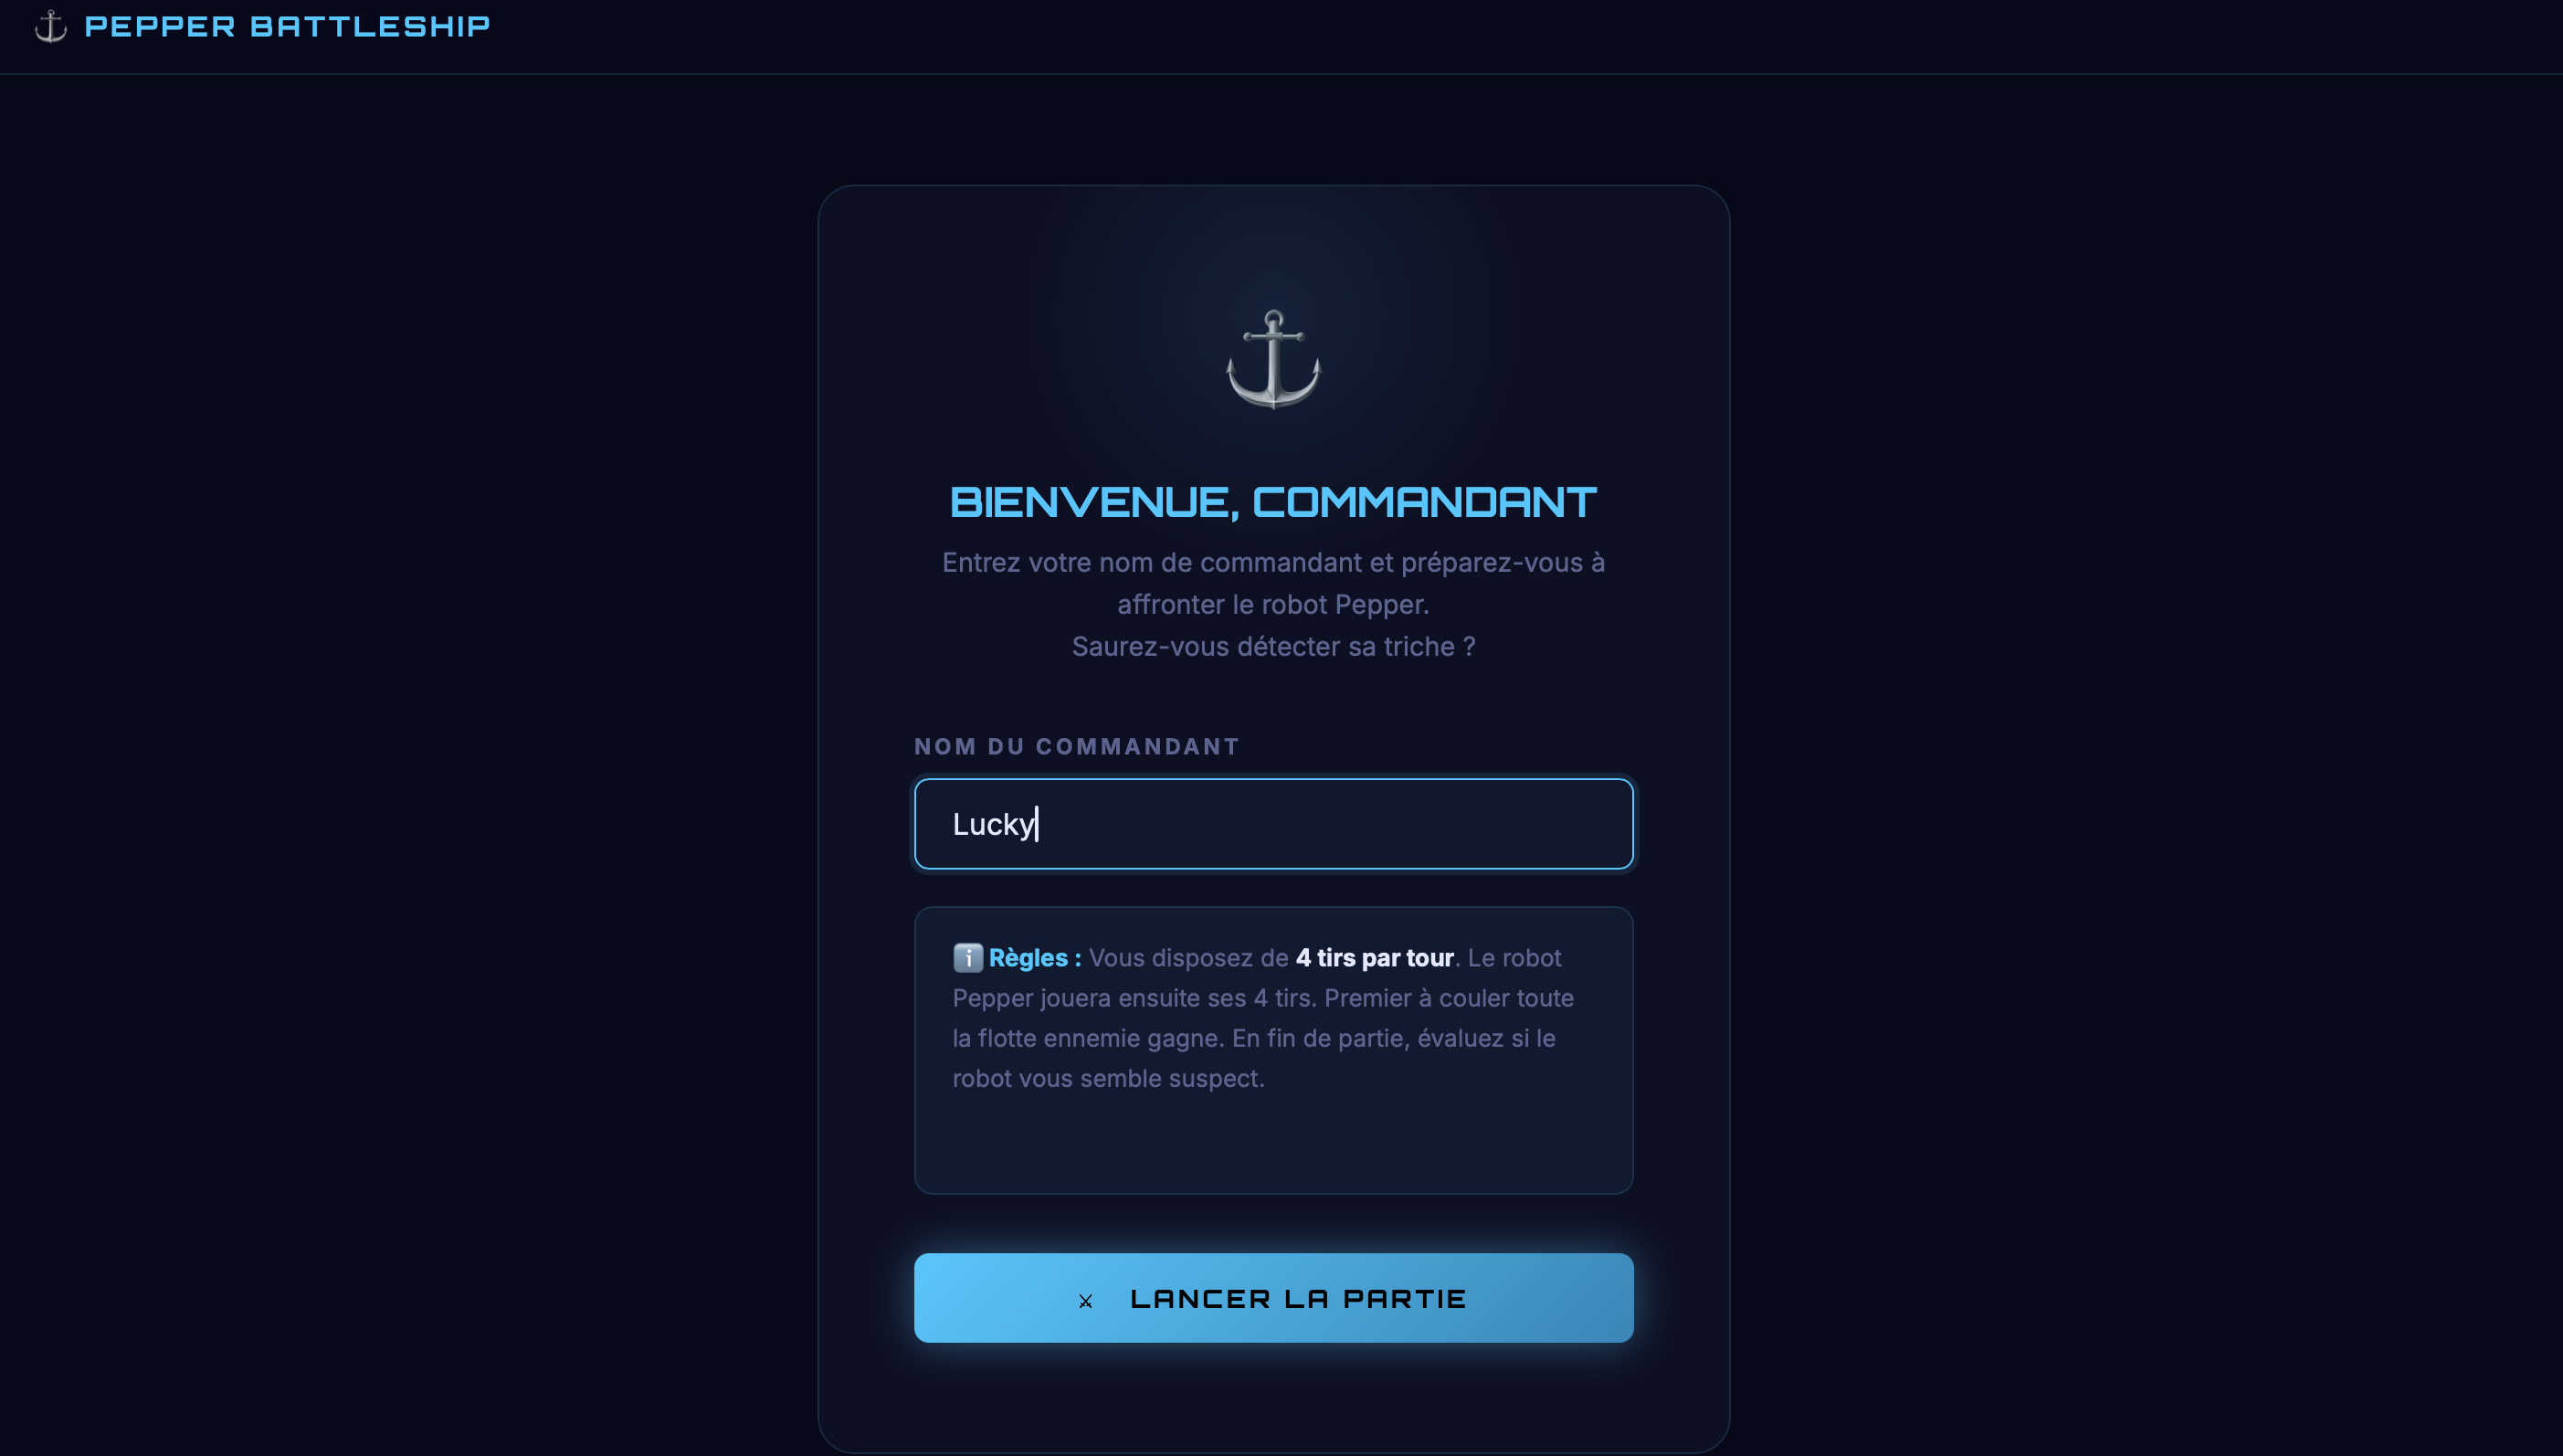
\includegraphics[width=0.85\textwidth]{../rapport/diagrams/interfaces_site/partie.png}
\end{center}
\end{frame}

\begin{frame}
\frametitle{Système de notation de confiance}
\textbf{Après chaque tour du bot :}

\begin{center}
\Large \textit{``Dans quelle mesure pensez-vous que le bot a triché ?''}
\end{center}

\vspace{0.5cm}

\begin{tabular}{c|l}
\textbf{Score} & \textbf{Interprétation} \\
\hline
0 & Pas du tout triché \\
1-2 & Peu probable \\
3 & Incertain \\
4-5 & Très suspect / Certainement triché \\
\end{tabular}

\vspace{0.5cm}
\begin{center}
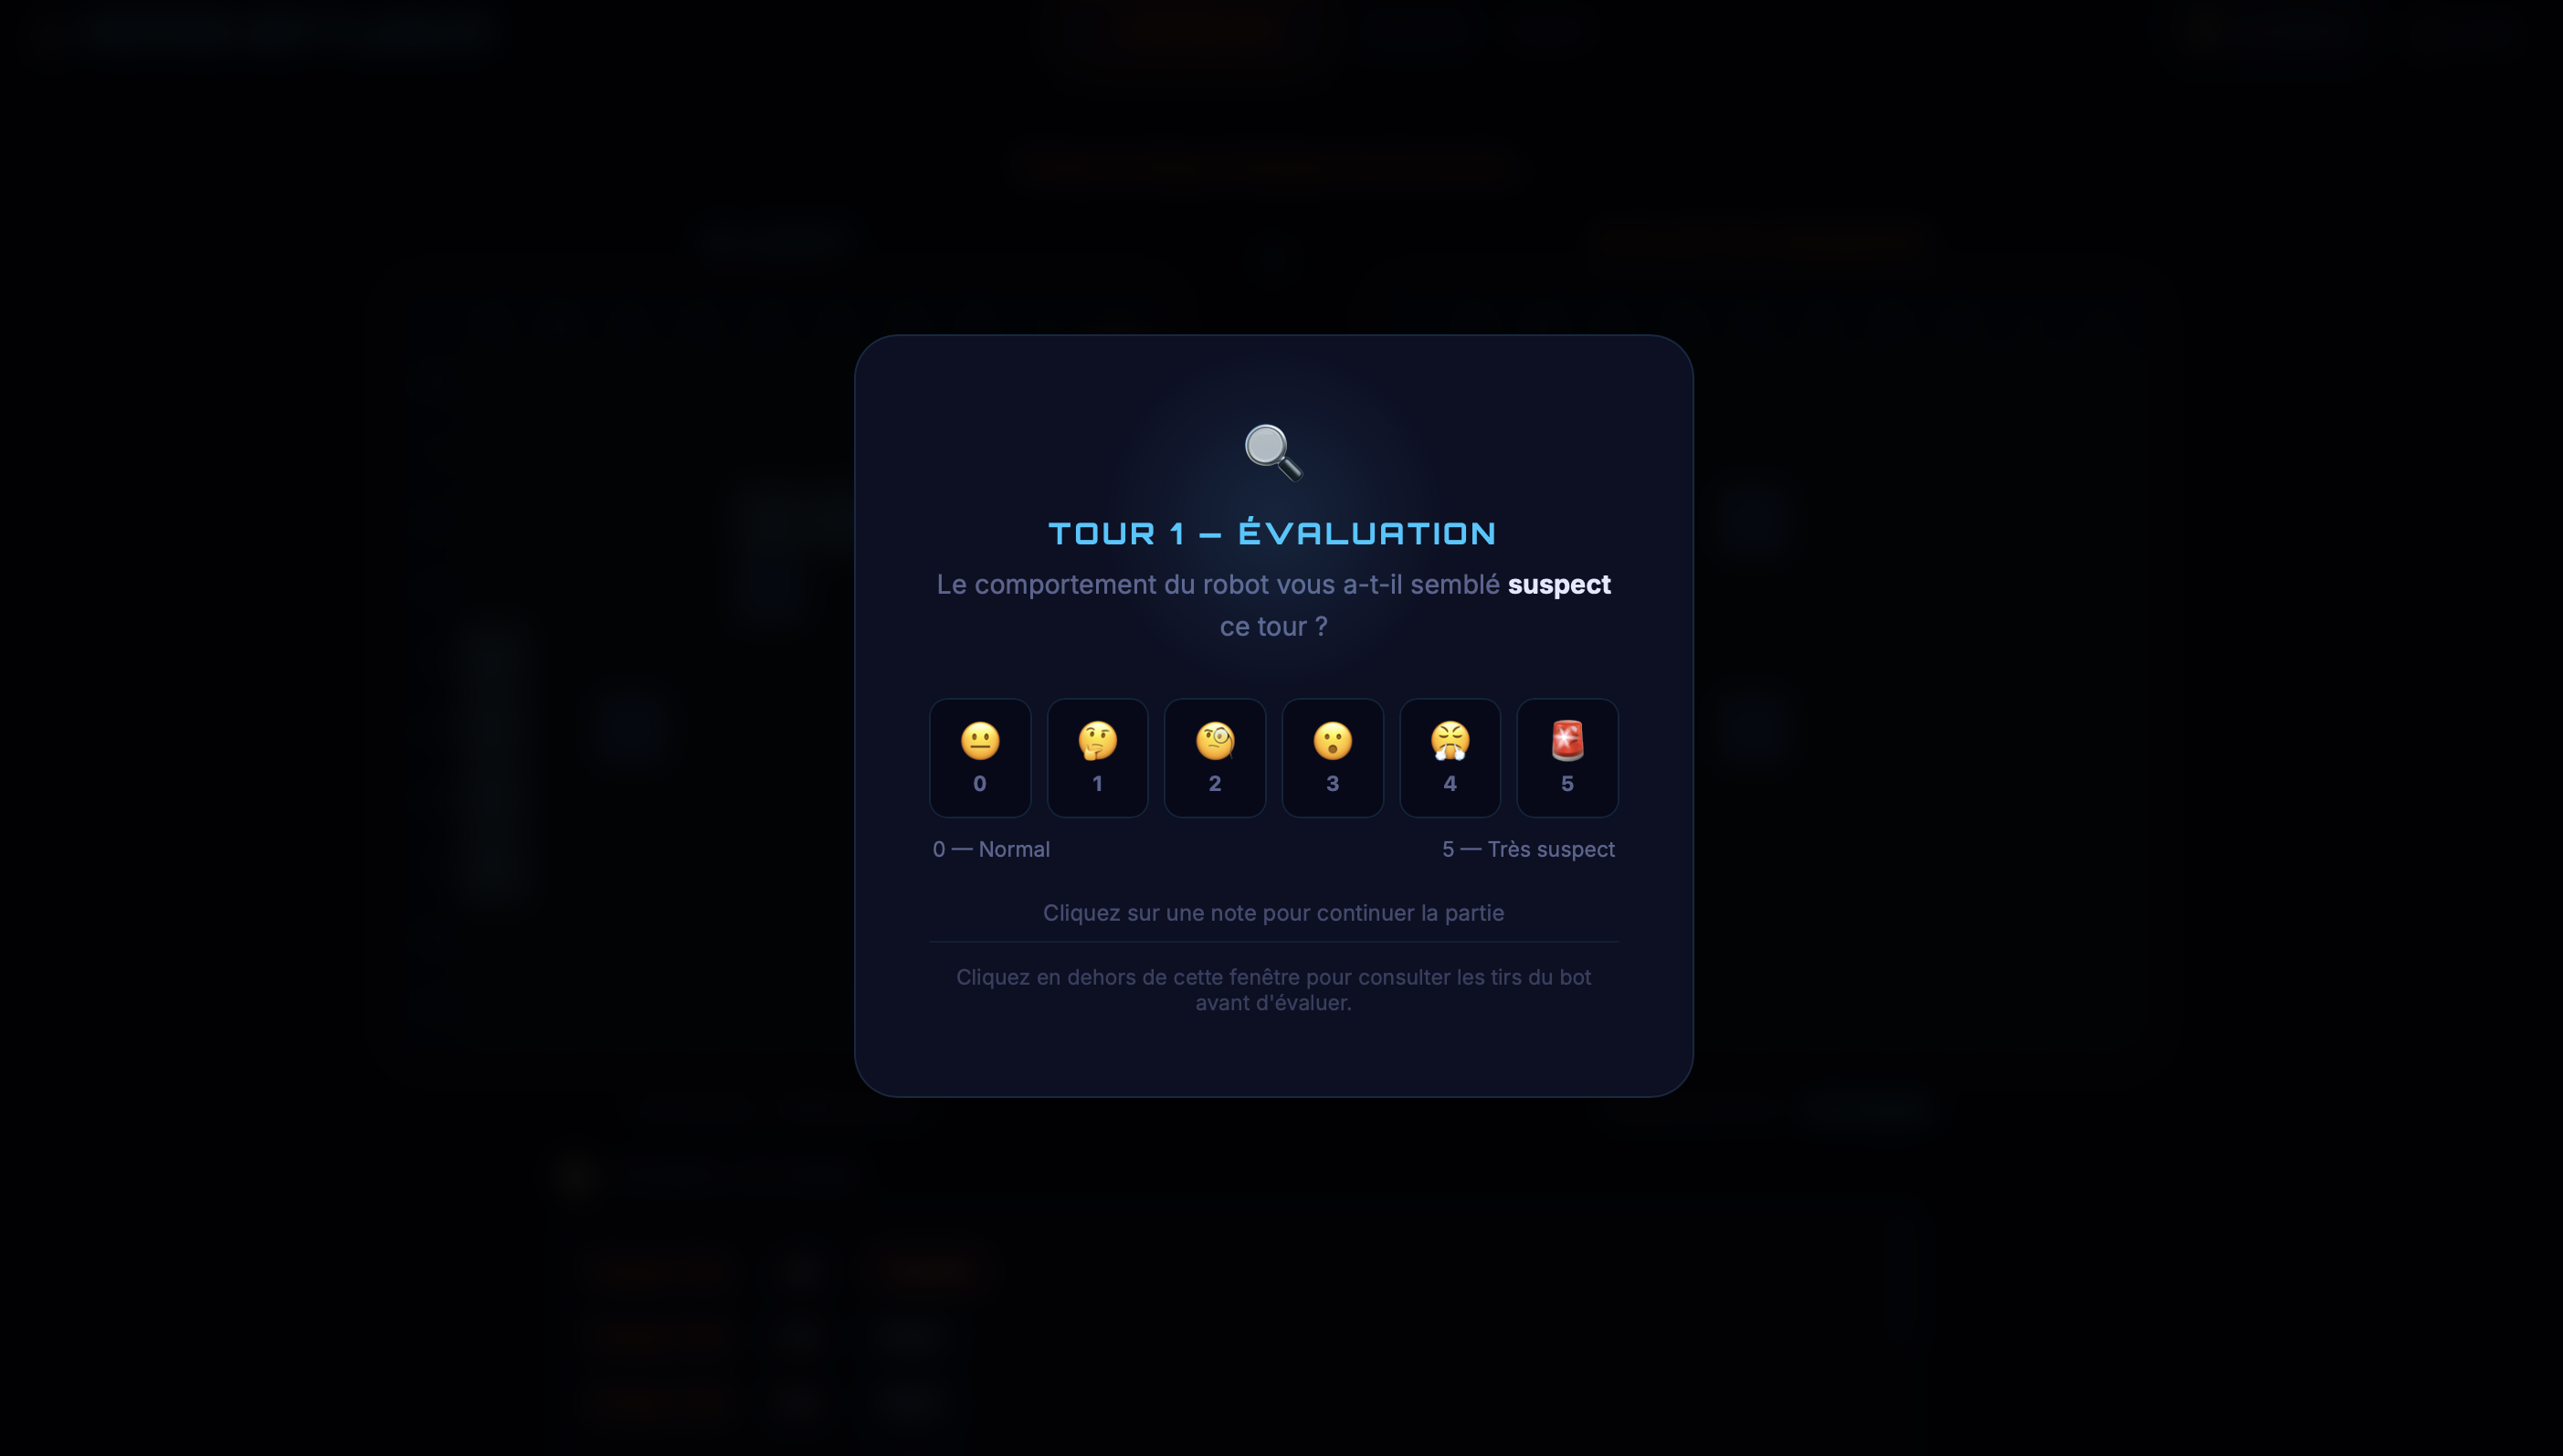
\includegraphics[width=0.70\textwidth]{../rapport/diagrams/interfaces_site/partie3.png}
\end{center}
\end{frame}

\begin{frame}
\frametitle{API REST}
\textbf{Routes principales :}
\begin{itemize}
    \item \texttt{GET /} : Landing page
    \item \texttt{POST /api/game/new} : Créer partie
    \item \texttt{POST /api/game/\{id\}/shoot} : Tir joueur
    \item \texttt{POST /api/game/\{id\}/bot-turn} : Tour du bot
    \item \texttt{POST /api/game/\{id\}/turn-trust} : Enregistrer score
    \item \texttt{GET /api/stats} : Statistiques globales
\end{itemize}

\vspace{0.5cm}
\begin{center}
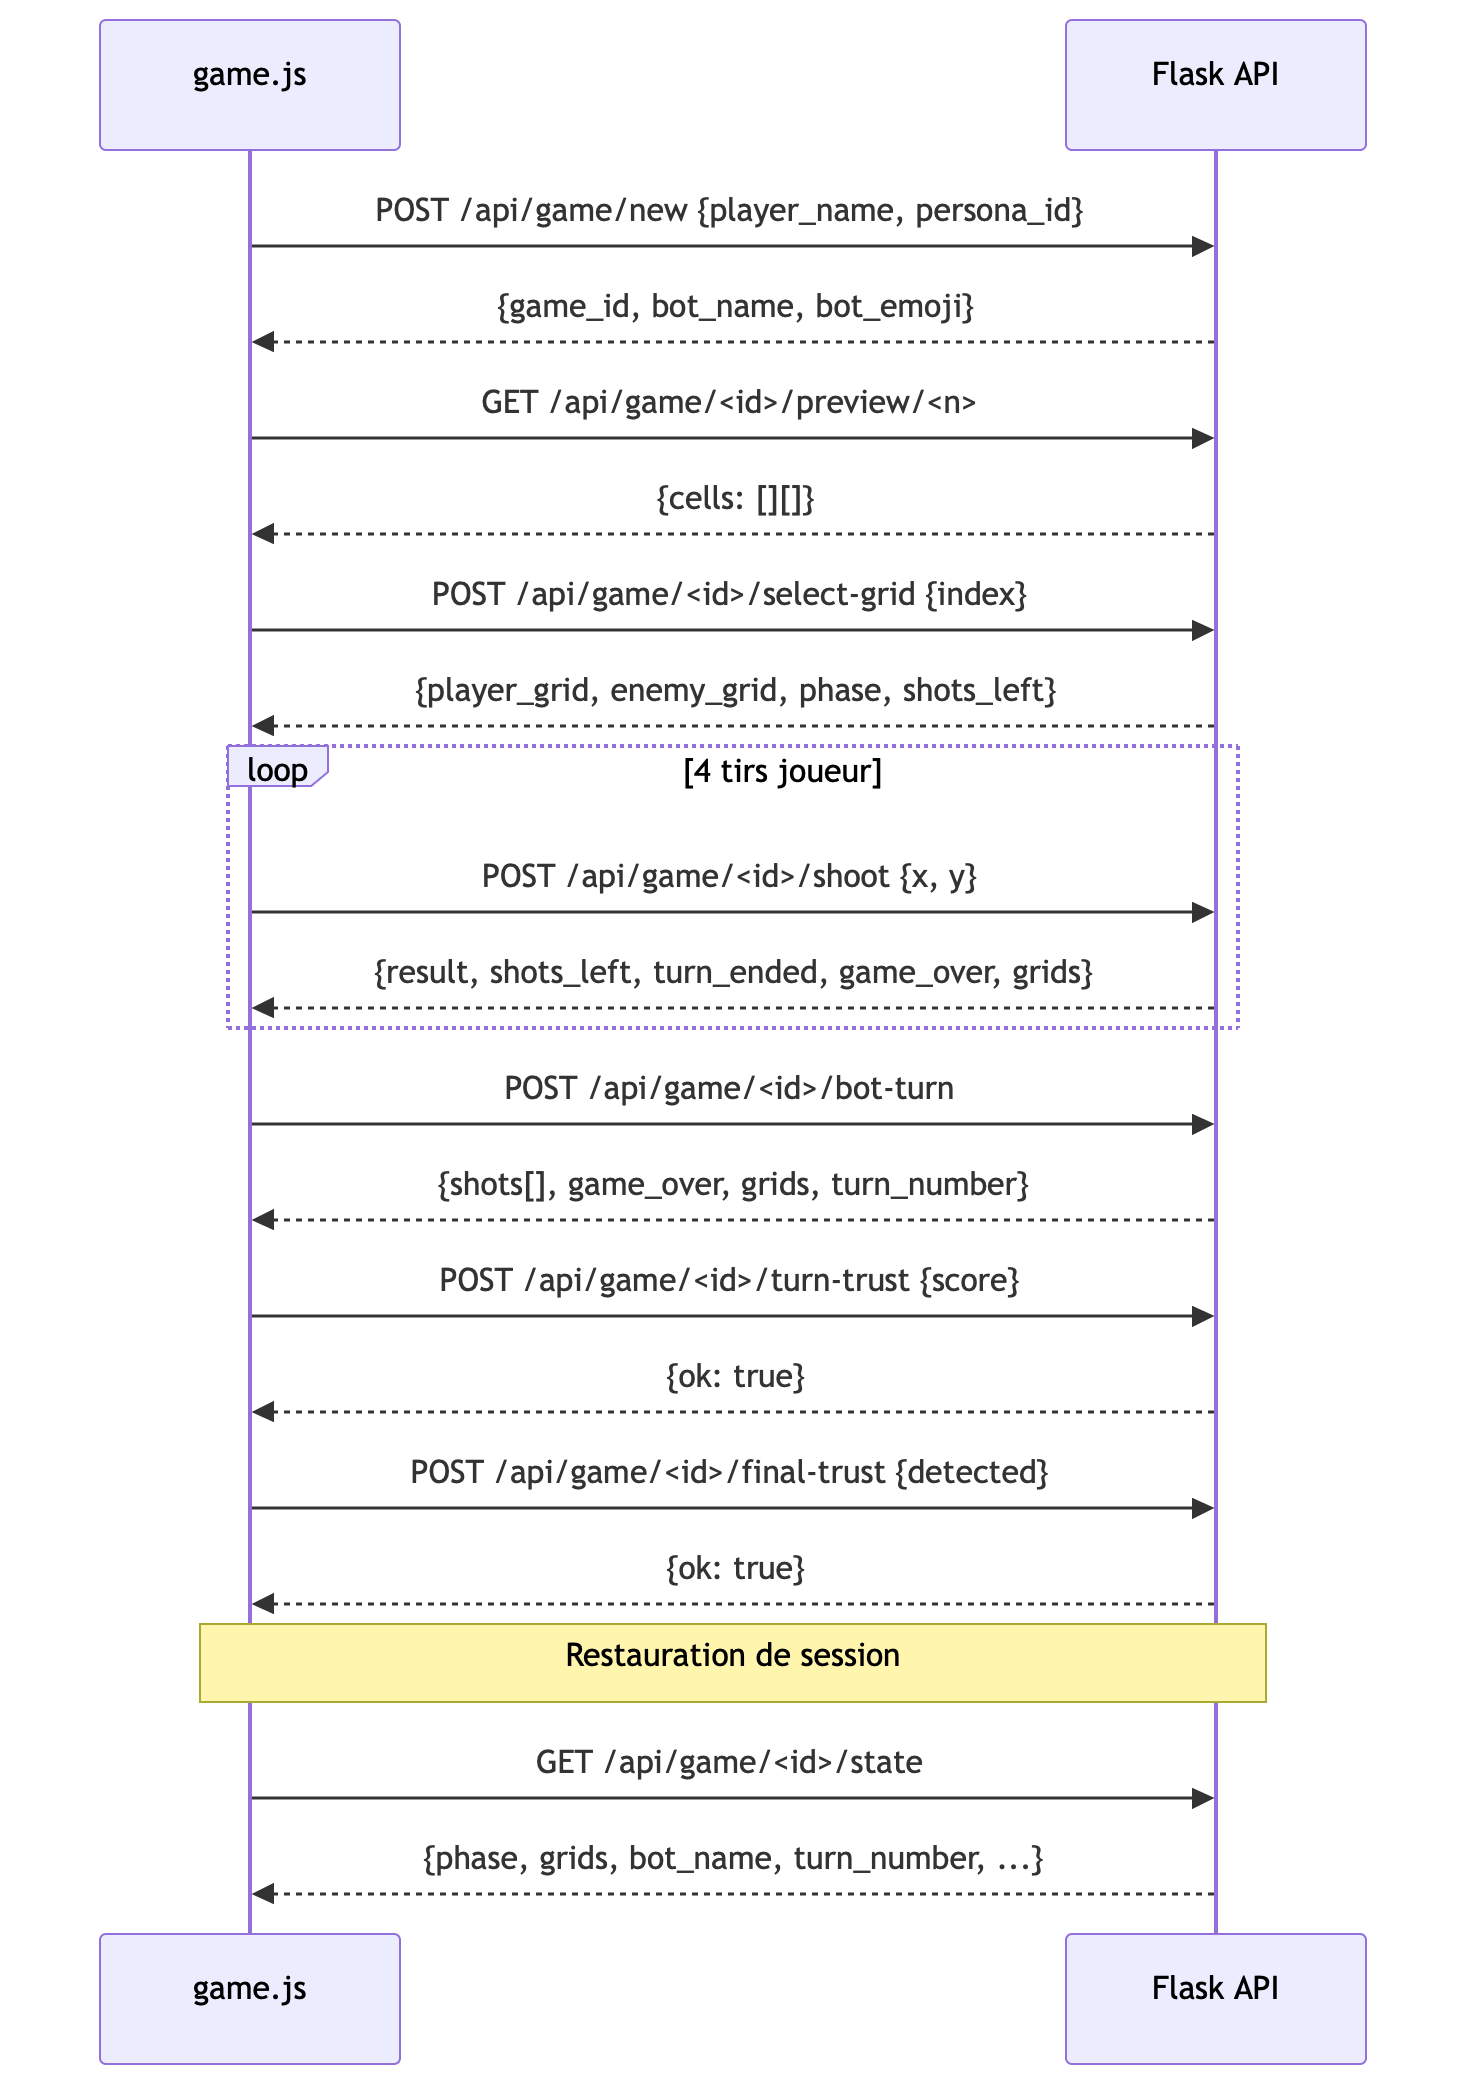
\includegraphics[width=0.80\textwidth]{../rapport/diagrams/images/Front/APIS.png}
\end{center}
\end{frame}

\subsection{Application Python}

\begin{frame}
\frametitle{Architecture modulaire Python}
\begin{center}
\placeholder{0.9\textwidth}{Schéma : Arborescence des modules}
\end{center}

\vspace{0.3cm}

\textbf{6 modules principaux :}
\begin{enumerate}
    \item \texttt{game\_logic/} - Moteur de jeu
    \item \texttt{classes/} - Modèles de données
    \item \texttt{players/} - Implémentations joueurs
    \item \texttt{interface/} - UI (Console + Tkinter)
    \item \texttt{database/} - Persistance SQLite
    \item \texttt{client/} - Communication réseau
\end{enumerate}
\end{frame}

\begin{frame}
\frametitle{GameMaster (Orchestrateur principal)}
\begin{center}
\placeholder{0.85\textwidth}{Schéma : Rôles et responsabilités du GameMaster}
\end{center}

\vspace{0.3cm}

\textbf{4 responsabilités :}
\begin{enumerate}
    \item Initialisation des joueurs (humain vs CheatBot)
    \item Gestion des tours de jeu
    \item Attribution des quotas de triche
    \item Enregistrement en base de données
\end{enumerate}
\end{frame}

\begin{frame}
\frametitle{CheatBot : Architecture de triche}
\textbf{Le cœur du protocole expérimental}

\vspace{0.5cm}

\textbf{Processus par tour :}
\begin{enumerate}
    \item Accès à la grille ennemie (si mode digital)
    \item Identification des cases de bateaux non touchées
    \item Sélection de $N$ cases bateaux (succès)
    \item Sélection de $4-N$ cases vides (échecs)
    \item Mélange aléatoire (éviter patterns)
    \item Exécution des 4 tirs
\end{enumerate}

\vspace{0.5cm}
\begin{center}
\placeholder{0.75\textwidth}{Schéma : Algorithme execute\_turn du CheatBot}
\end{center}
\end{frame}

\begin{frame}
\frametitle{CheatBot : Quotas et équivalence}
\textbf{Garantie de contrôle expérimental :}

\begin{itemize}
    \item Quota prédéfini par tour (ex: [2, 1, 3, 2, 1, ...])
    \item \textbf{Même séquence} utilisée dans les deux conditions
    \item Adaptation automatique si moins de bateaux disponibles
    \item Communication socket optionnelle vers Pepper
\end{itemize}

\vspace{0.5cm}

\textbf{Résultat :} Comportement observable \textbf{strictement identique} dans les deux parties, seul le label varie.

\vspace{0.5cm}
\begin{center}
\placeholder{0.75\textwidth}{Schéma : Comparaison quotas Partie 1 vs Partie 2}
\end{center}
\end{frame}

\begin{frame}
\frametitle{Hiérarchie des joueurs}
\begin{center}
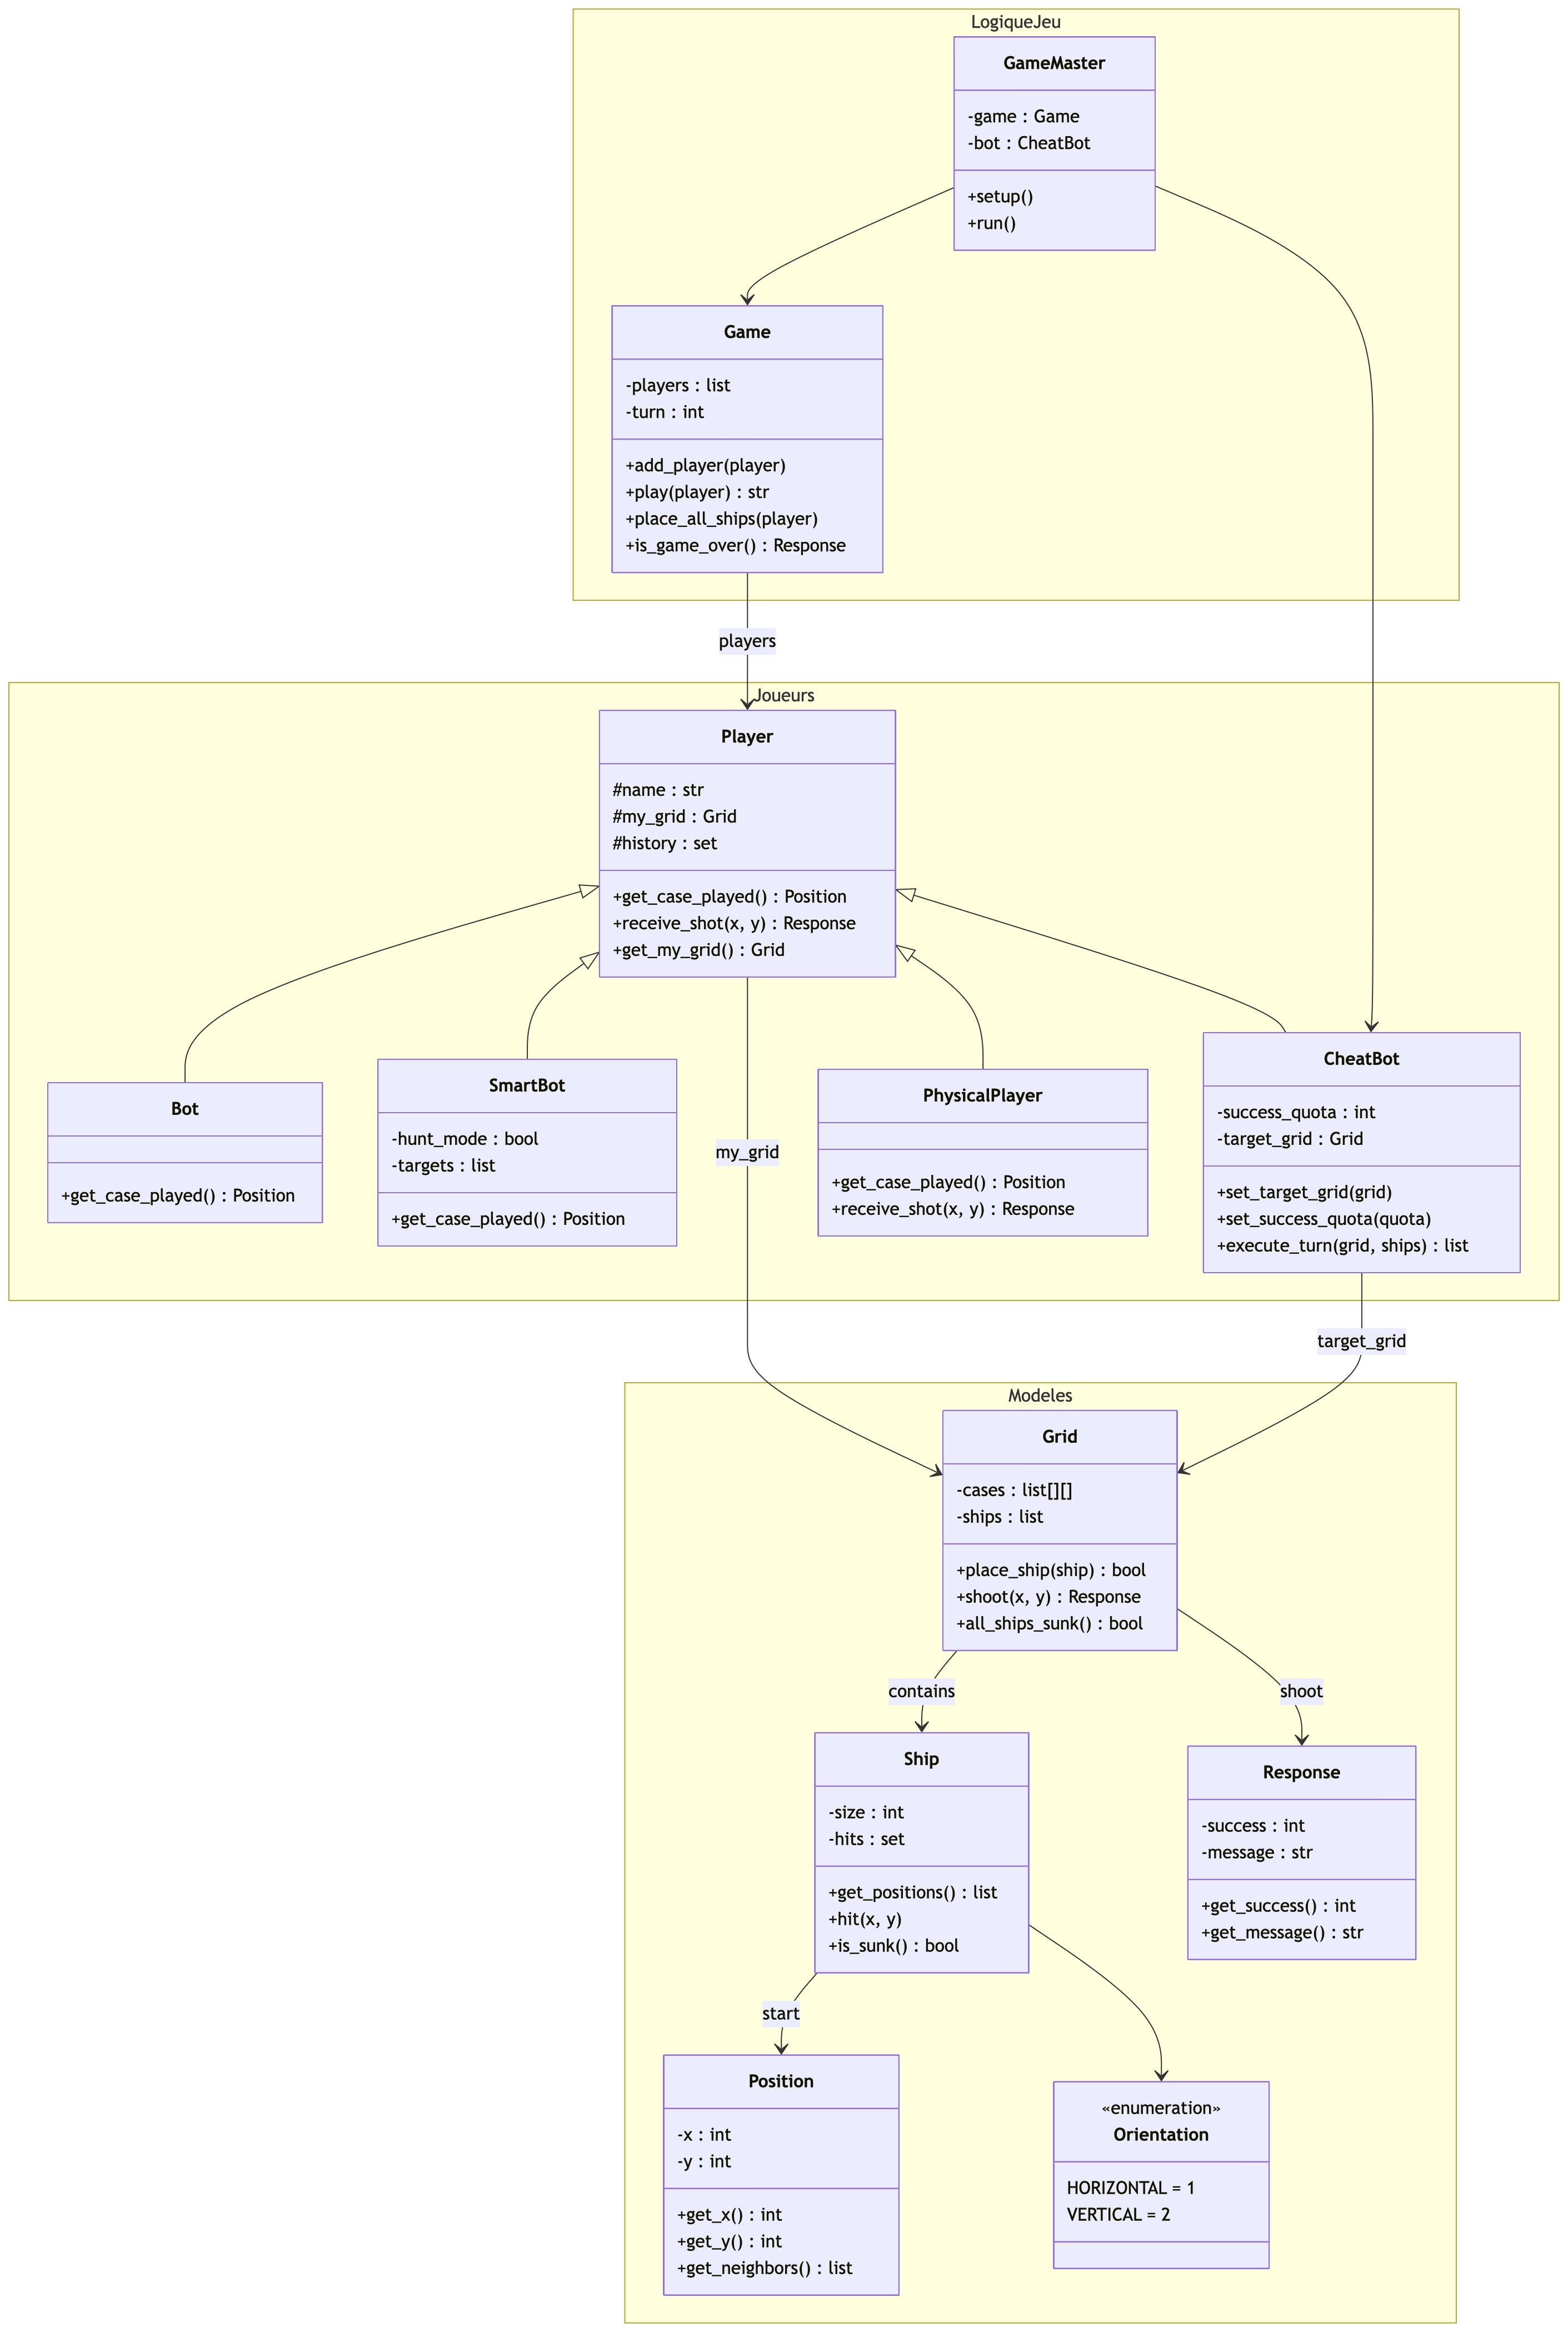
\includegraphics[width=0.90\textwidth]{../rapport/diagrams/images/diag_classes.png}
\end{center}

\vspace{0.3cm}

\begin{itemize}
    \item \textbf{Player} (classe de base) : Grilles, historique, entrée utilisateur
    \item \textbf{CheatBot} : Triche discrète
    \item \textbf{SmartBot} : Stratégie heuristique
    \item \textbf{PhysicalPlayer} : Interface robot Pepper
\end{itemize}
\end{frame}

\begin{frame}
\frametitle{Modèles de données}
\begin{columns}[T]
\column{0.5\textwidth}
\textbf{Grid (10×10)}
\begin{itemize}
    \item Navires placés
    \item État de chaque case
    \item Méthode \texttt{shoot(x,y)}
\end{itemize}

\textbf{Ship}
\begin{itemize}
    \item Position, orientation
    \item Taille (5, 4, 3, 3, 2)
    \item Détection coulage
\end{itemize}

\column{0.5\textwidth}
\textbf{Position}
\begin{itemize}
    \item Coordonnées (x, y)
    \item Validation limites
\end{itemize}

\textbf{Response}
\begin{itemize}
    \item Message (touché/coulé/raté)
    \item État après tir
\end{itemize}
\end{columns}

\vspace{0.5cm}
\begin{center}
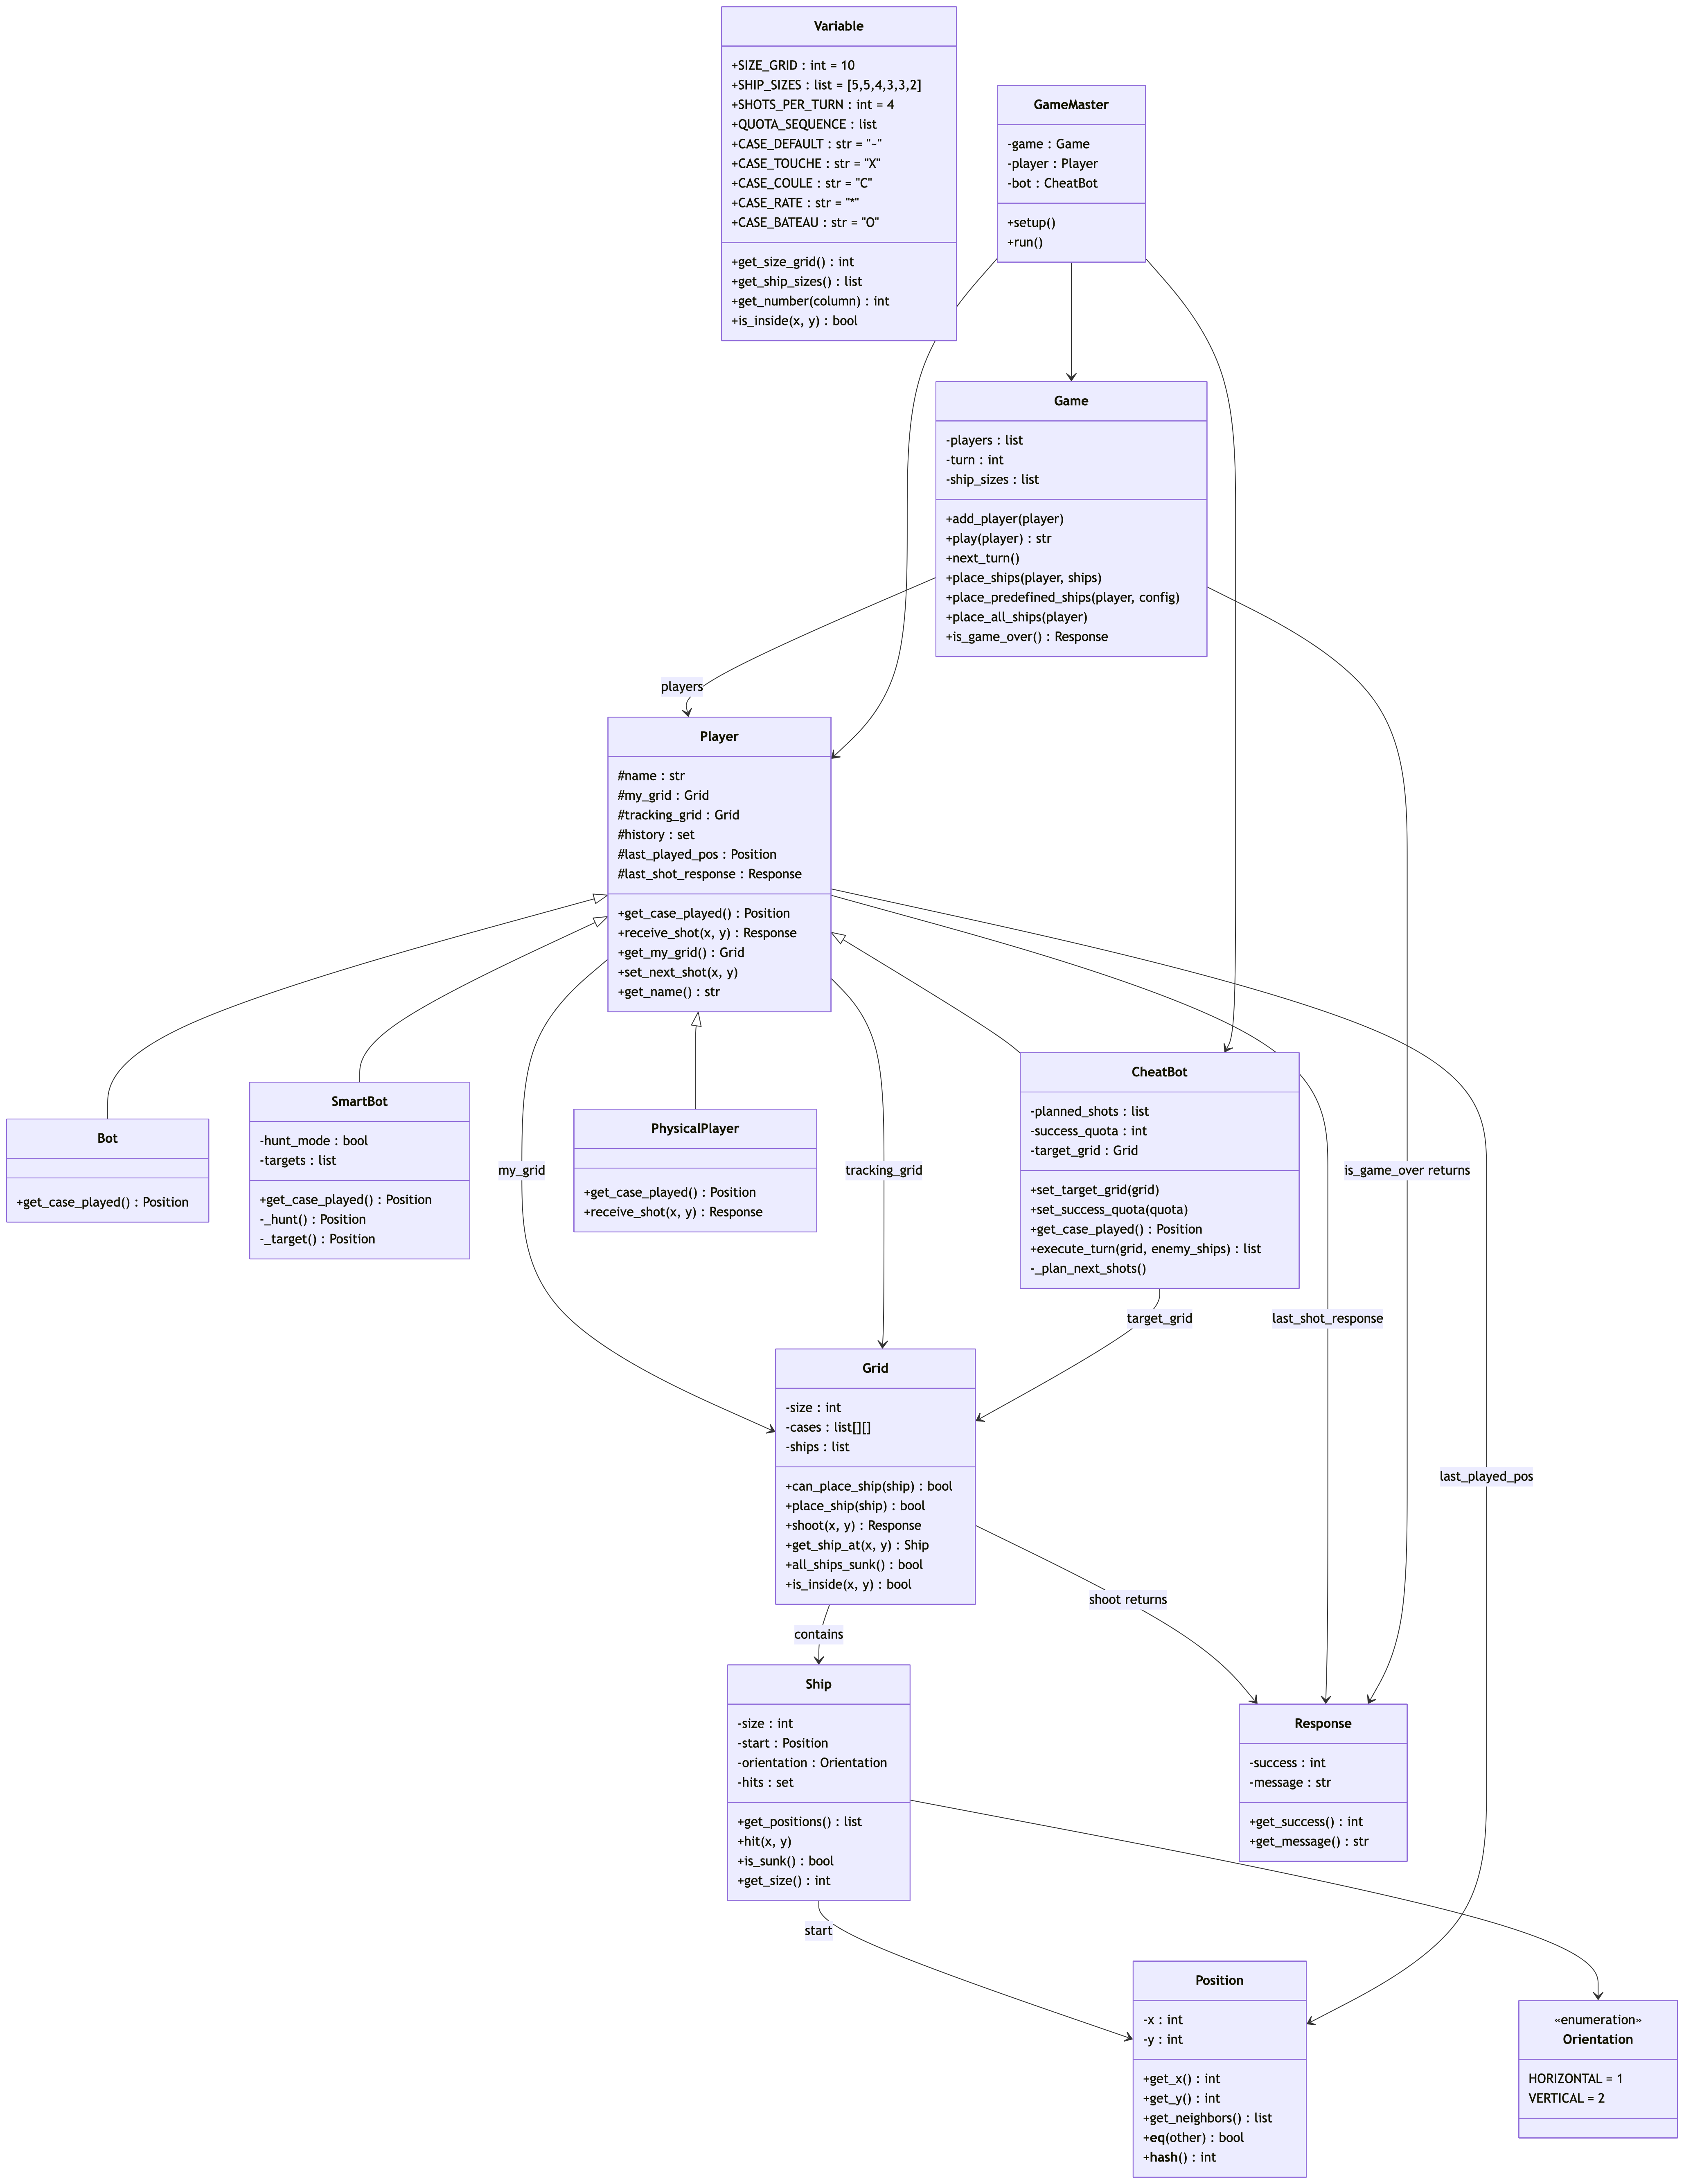
\includegraphics[width=0.80\textwidth]{../rapport/diagrams/images/classes.png}
\end{center}
\end{frame}

\begin{frame}
\frametitle{Base de données SQLite}
\textbf{Schéma relationnel :}

\begin{columns}[T]
\column{0.33\textwidth}
\textbf{Table Game}
\begin{itemize}
    \item game\_id (PK)
    \item player\_name
    \item player\_type
    \item date\_played
    \item winner
\end{itemize}

\column{0.33\textwidth}
\textbf{Table Turn}
\begin{itemize}
    \item turn\_id (PK)
    \item game\_id (FK)
    \item turn\_number
    \item bot\_quota
    \item trust\_score
\end{itemize}

\column{0.33\textwidth}
\textbf{Table BotShot}
\begin{itemize}
    \item shot\_id (PK)
    \item turn\_id (FK)
    \item shot\_number
    \item pos\_x, pos\_y
    \item result
\end{itemize}
\end{columns}

\vspace{0.5cm}
\begin{center}
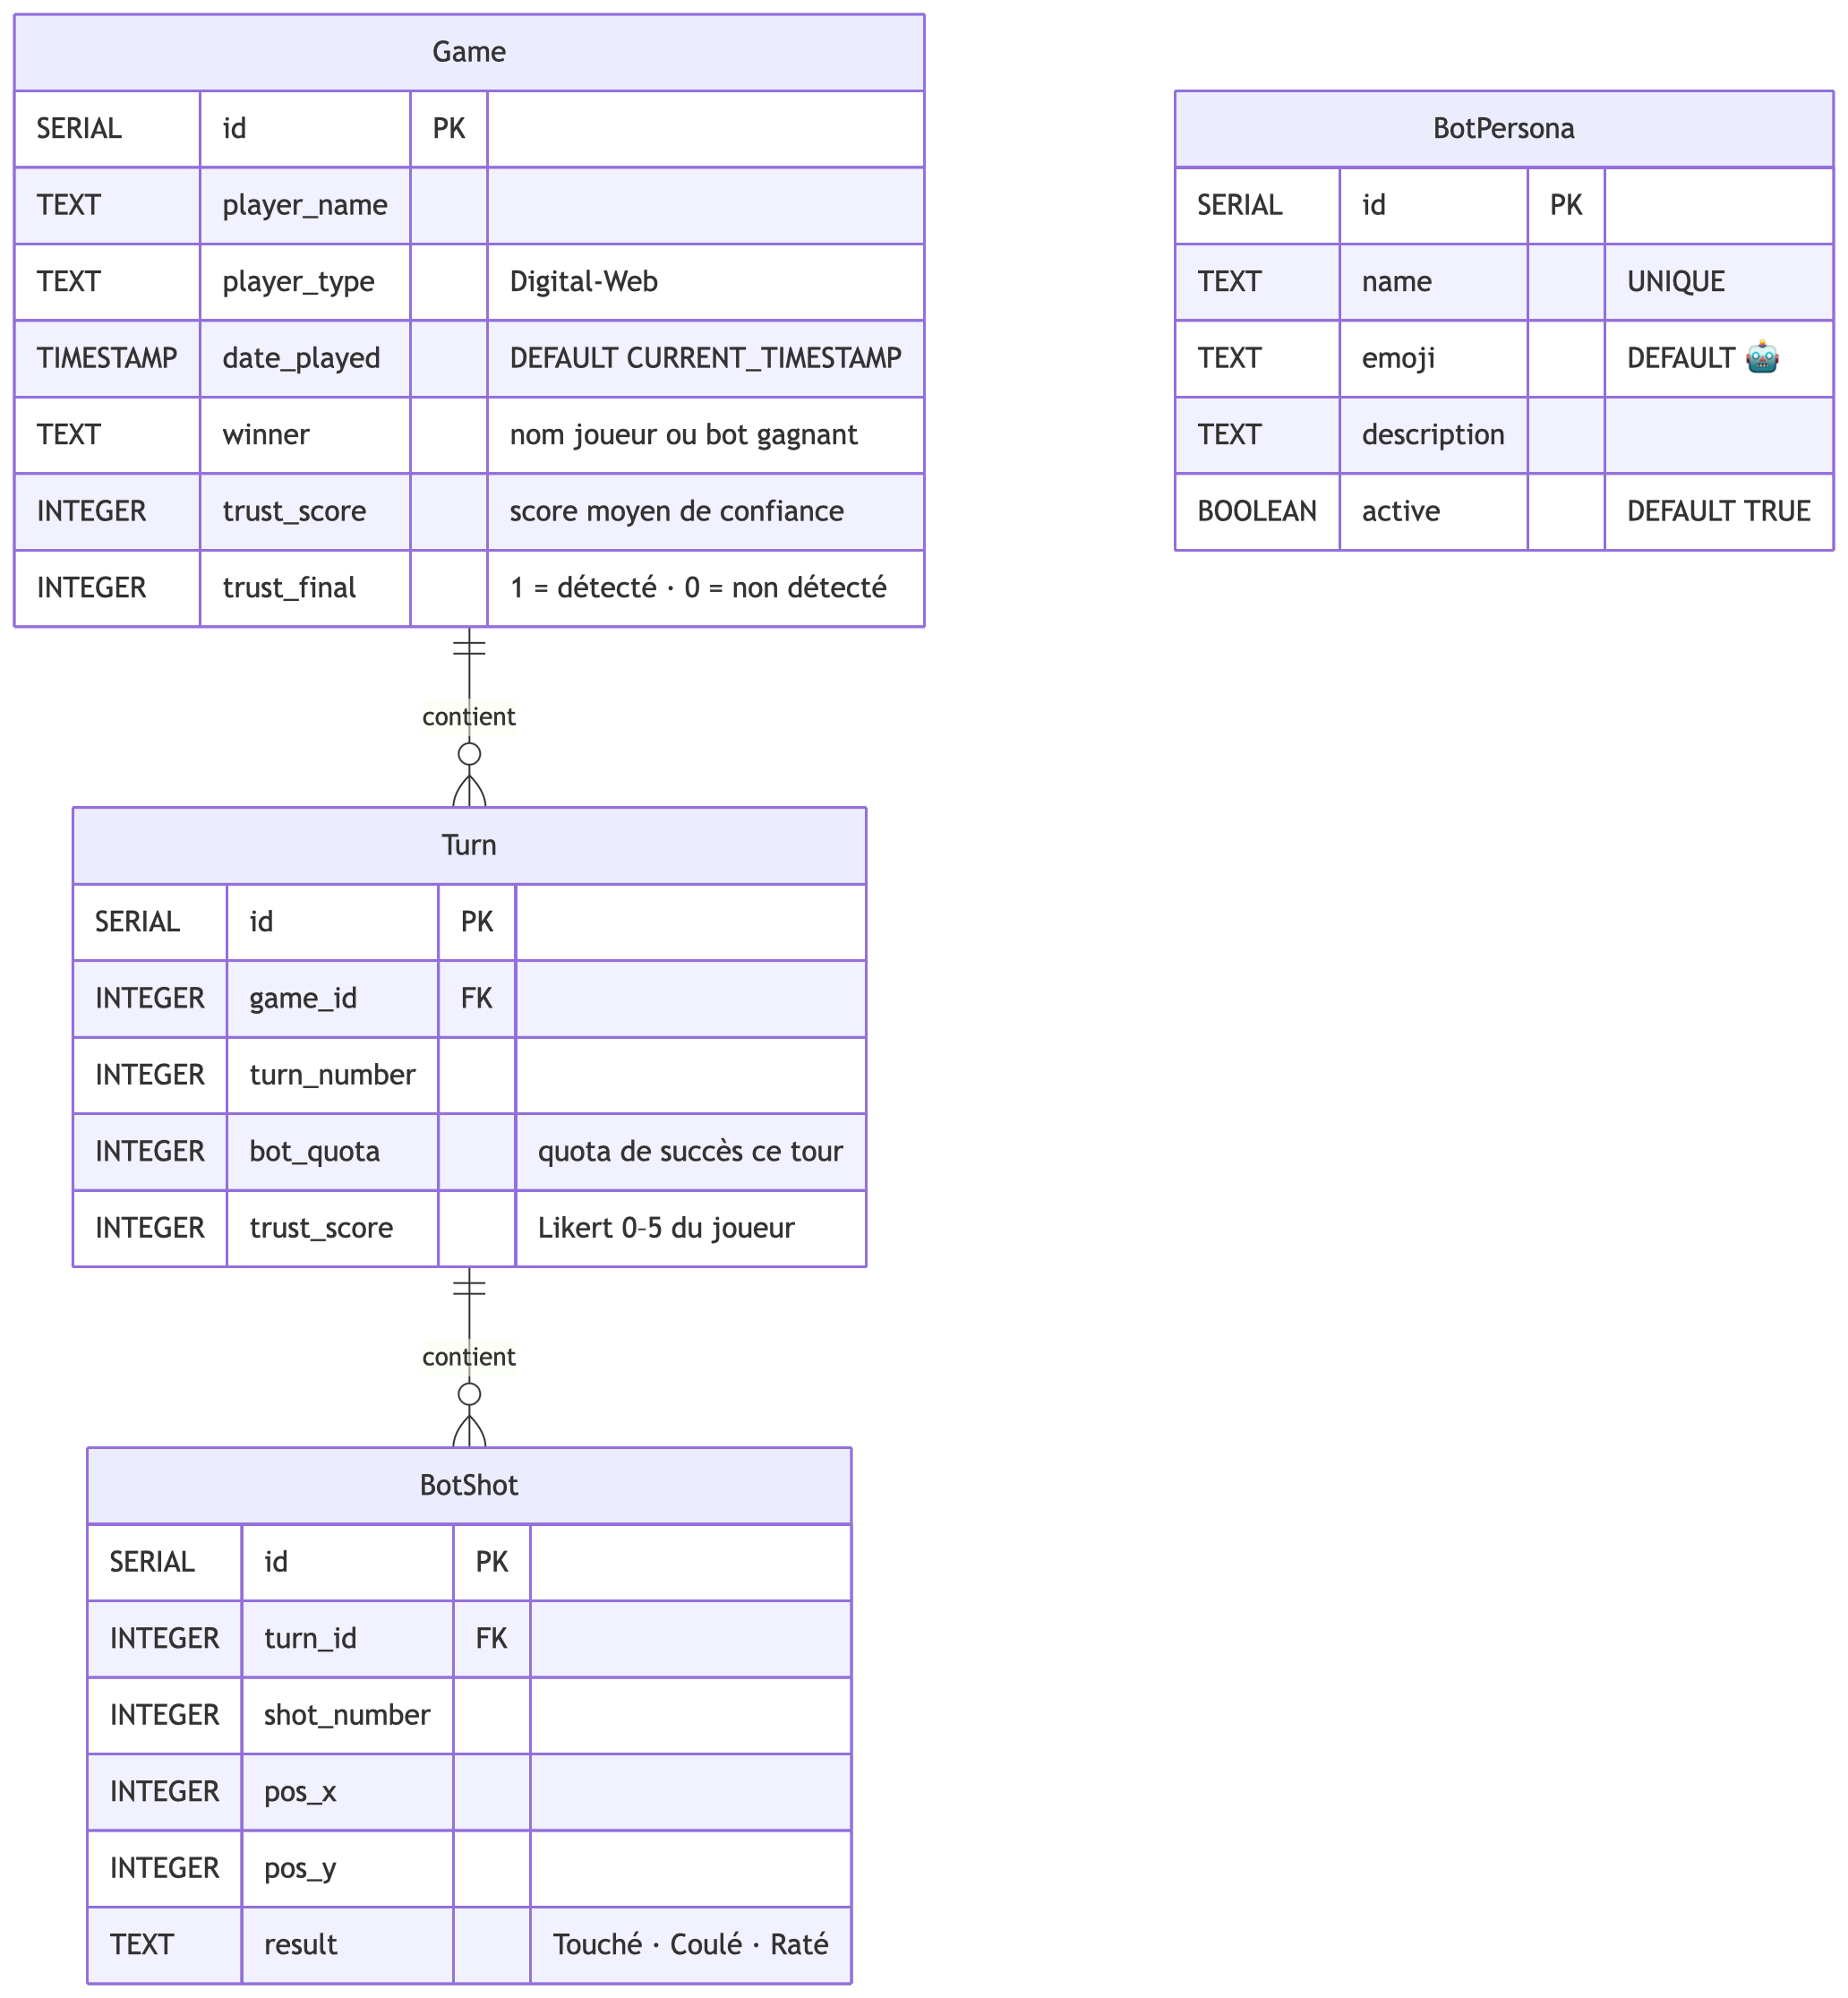
\includegraphics[width=0.78\textwidth]{../rapport/diagrams/images/Bdd.png}
\end{center}
\end{frame}

\begin{frame}
\frametitle{Interfaces utilisateur}
\begin{columns}[T]
\column{0.5\textwidth}
\textbf{Mode Console}
\begin{itemize}
    \item Affichage textuel
    \item Interaction CLI
    \item Tests et développement
\end{itemize}

\column{0.5\textwidth}
\textbf{Mode Graphique (Tkinter)}
\begin{itemize}
    \item Canvases 10×10
    \item Visualisation intuitive
    \item Intégration questionnaire
\end{itemize}
\end{columns}

\vspace{1cm}
\begin{center}
\placeholder{0.8\textwidth}{Capture d'écran : Interface Tkinter}
\end{center}
\end{frame}

\subsection{Intégration Web $\leftrightarrow$ Python}

\begin{frame}
\frametitle{Synchronisation Web $\leftrightarrow$ Python}
\textbf{Flux de données complet :}

\begin{enumerate}
    \item Utilisateur accède à \texttt{/game} (Flask)
    \item Flask initialise GameMaster en Python
    \item Tirs joueur → API \texttt{/shoot} → logique Python
    \item Tour du bot → appel CheatBot.get\_case\_played()
    \item Résultats → enregistrement SQLite
    \item Scores de confiance → base de données
\end{enumerate}

\vspace{0.5cm}
\begin{center}
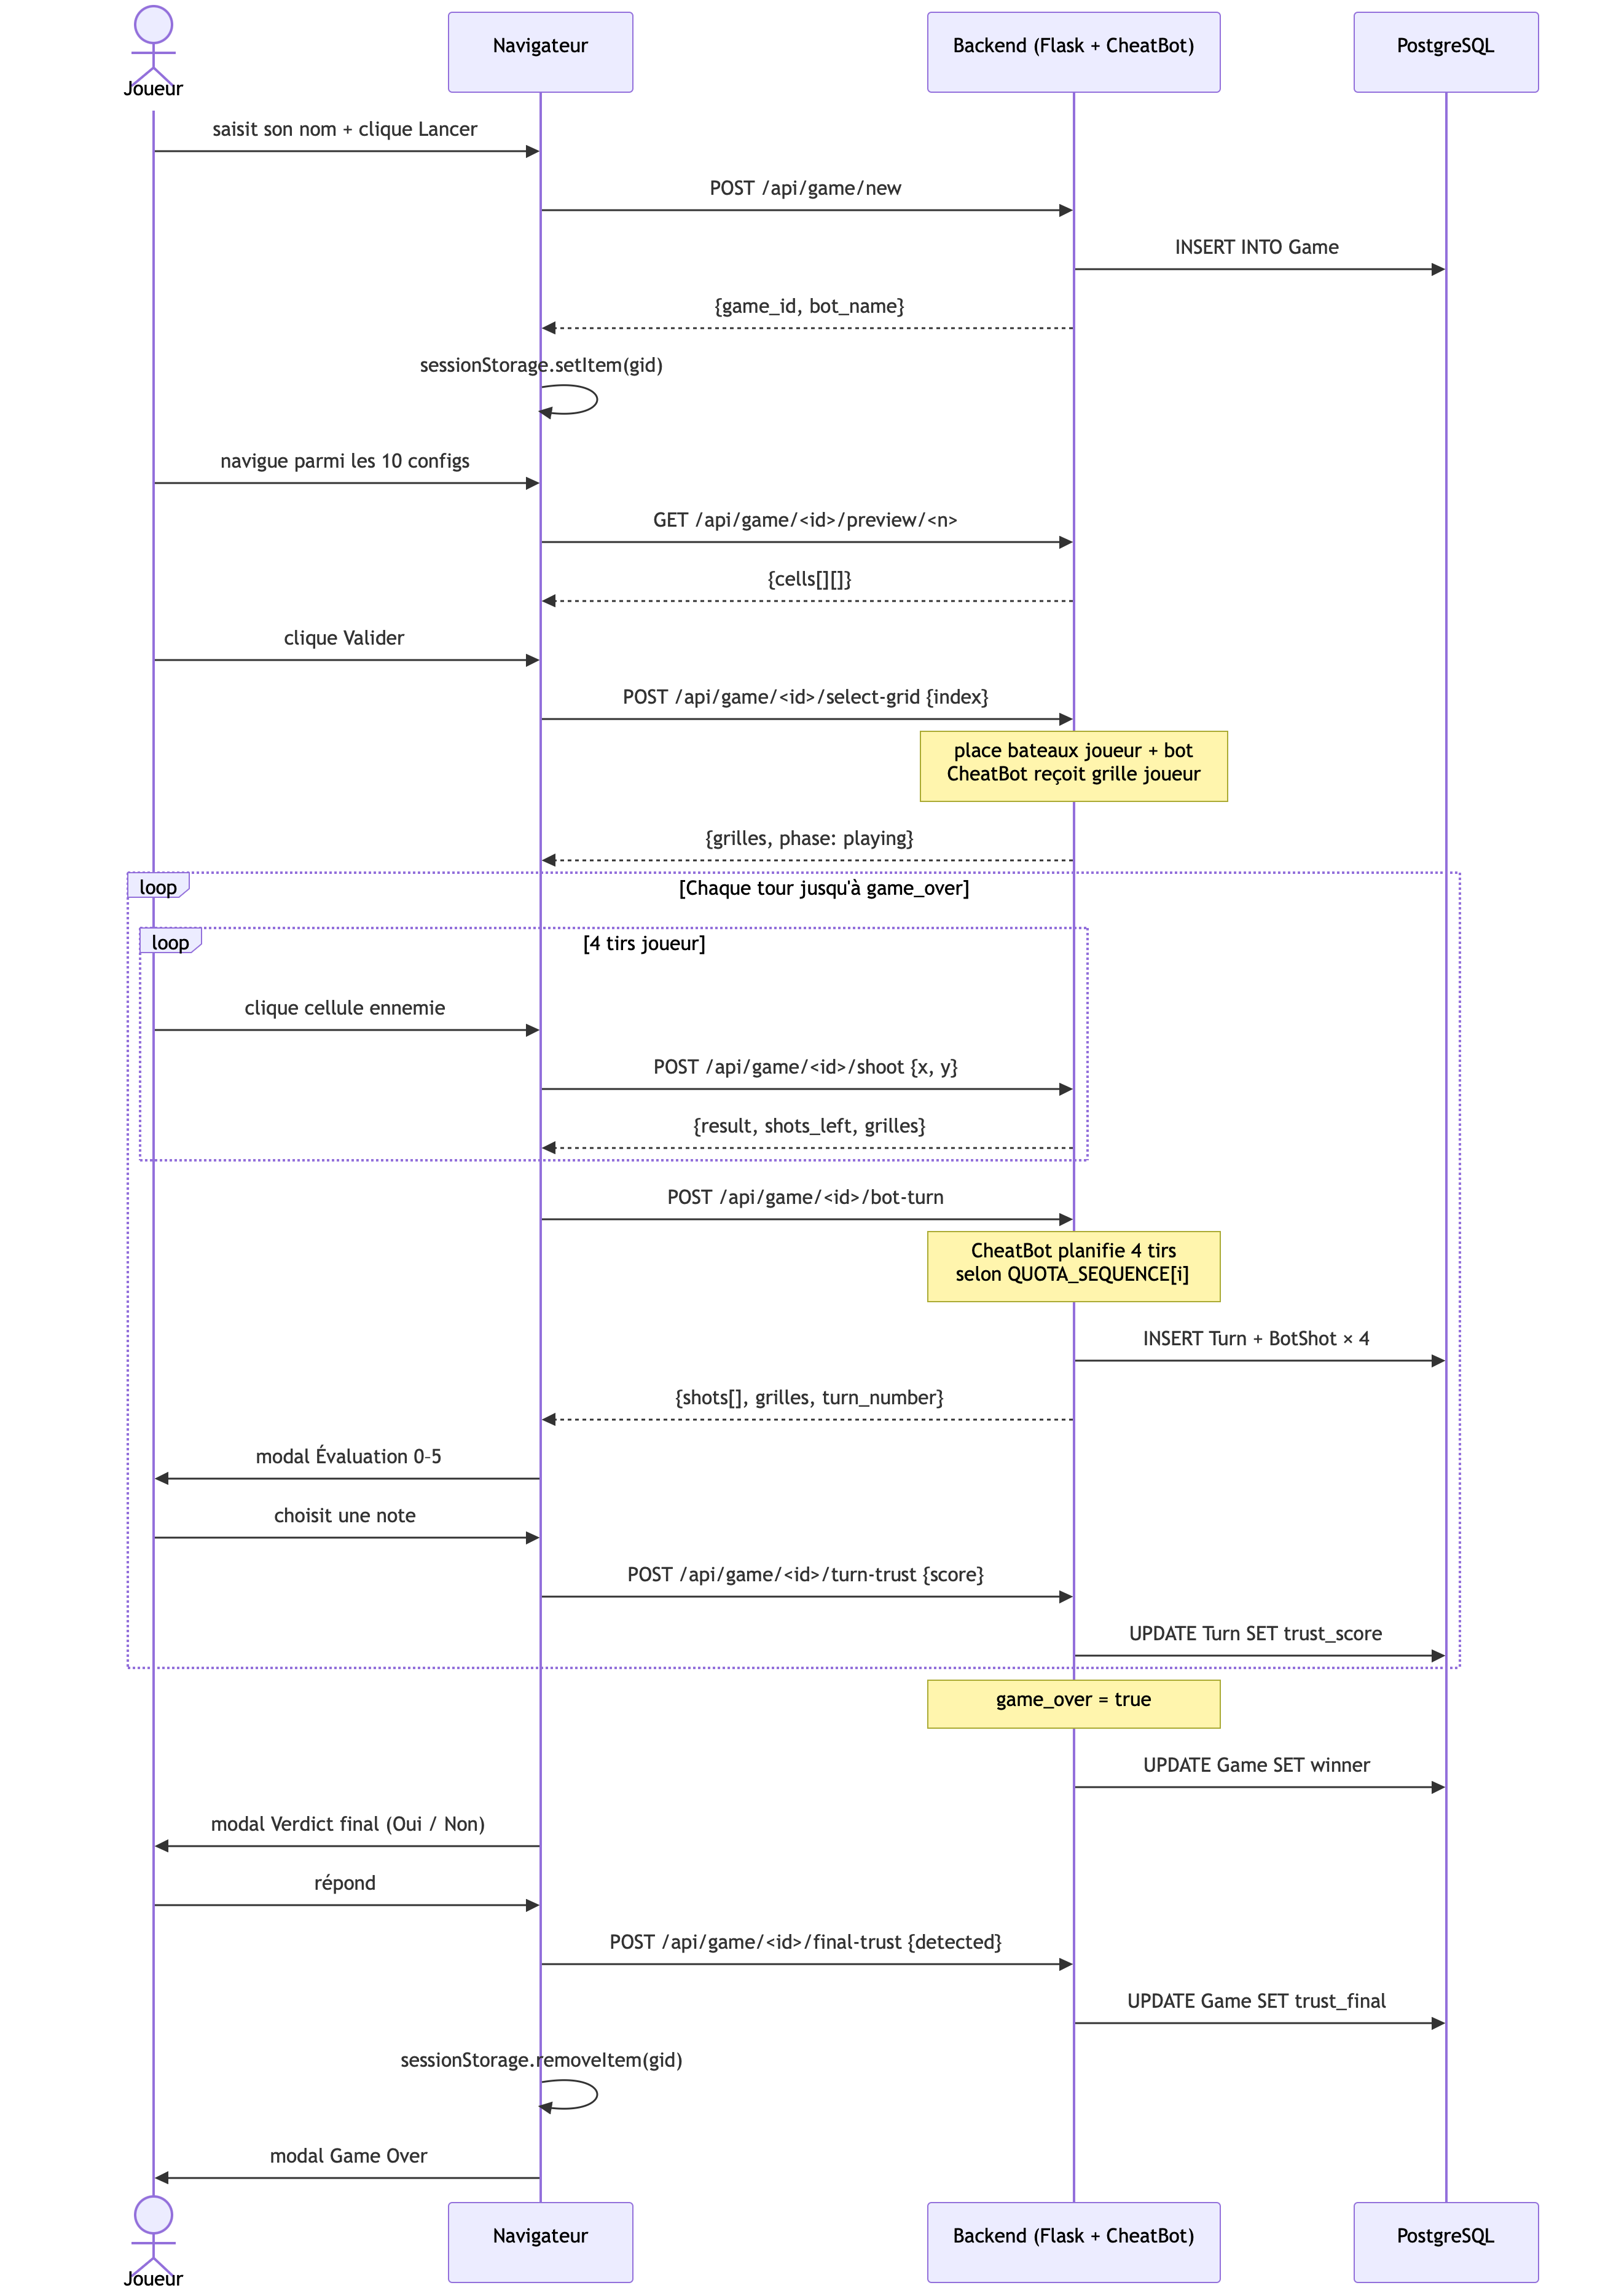
\includegraphics[width=0.85\textwidth]{../rapport/diagrams/images/SequencePartie.png}
\end{center}
\end{frame}

\begin{frame}
\frametitle{Avantages de cette architecture}
\begin{itemize}
    \item \textbf{Interface moderne} : Web pour UX optimale et recrutement en ligne
    \item \textbf{Logique robuste} : Python éprouvé et testé
    \item \textbf{Contrôle rigoureux} : Comportement identique dans les deux conditions
    \item \textbf{Reproductibilité} : Code centralisé et versionné
    \item \textbf{Scalabilité} : Collecte de données auprès de nombreux participants
    \item \textbf{Flexibilité future} : Intégration possible avec Pepper (socket TCP/IP)
\end{itemize}
\end{frame}

% ═════════════════════════════════════════════════════════════════════════
% SECTION 4 : PROTOCOLE EXPÉRIMENTAL
% ═════════════════════════════════════════════════════════════════════════

\section{Protocole Expérimental}

\begin{frame}
\frametitle{Design quasi-expérimental}
\textbf{Plan intra-groupe (within-subjects) :}

\begin{center}
Chaque participant joue \textbf{2 parties} avec comportement adversaire \textbf{identique}
\end{center}

\vspace{0.5cm}

\begin{tabular}{|c|c|c|}
\hline
& \textbf{Partie 1} & \textbf{Partie 2} \\
\hline
Condition A & Adversaire X (Label 1) & Adversaire Y (Label 2) \\
\hline
Condition B & Adversaire Y (Label 2) & Adversaire X (Label 1) \\
\hline
\end{tabular}

\vspace{0.5cm}

Label 1 = Humain (adversaire présenté comme joueur humain)

Label 2 = IA (adversaire présenté comme CheatBot)

\vspace{0.5cm}
\begin{center}
\placeholder{0.7\textwidth}{Schéma : Contrebalancement des conditions}
\end{center}
\end{frame}

\begin{frame}
\frametitle{Déroulement des parties}
\textbf{Phases d'une partie :}
\begin{enumerate}
    \item Sélection du nom du joueur
    \item \todo{[Questionnaire démographique - À préciser]}
    \item Sélection de la configuration de flotte (10 grilles prédéfinies)
    \item Combat (alternance joueur $\leftrightarrow$ bot, 4 tirs/tour)
    \item Évaluation de confiance après chaque tour du bot (0-5)
    \item Fin : Victoire ou défaite
    \item \todo{[Questionnaire post-expérience - À développer]}
\end{enumerate}

\vspace{0.5cm}
\begin{center}
\placeholder{0.75\textwidth}{Timeline : Déroulement temporel d'une partie}
\end{center}
\end{frame}

\begin{frame}
\frametitle{Mesure de confiance}
\textbf{Variable dépendante principale :}

\vspace{0.5cm}

À la fin de chaque tour du bot, le joueur répond :

\begin{center}
\Large \textit{``Dans quelle mesure pensez-vous que votre adversaire a triché ?''}
\end{center}

\vspace{0.5cm}

Échelle de Likert 0-5 :
\begin{itemize}
    \item 0 = Pas du tout triché
    \item 1-2 = Peu probable
    \item 3 = Incertain
    \item 4-5 = Très suspect / Certainement triché
\end{itemize}

\vspace{0.5cm}
\textbf{Enregistrement :} Horodaté et stocké immédiatement en base
\end{frame}

\begin{frame}
\frametitle{Variables contrôlées}
\textbf{Garantie d'équivalence comportementale :}

\begin{itemize}
    \item \textbf{Même adversaire} : Code CheatBot identique
    \item \textbf{Même quota} : Séquence [q1, q2, ..., qN] répétée
    \item \textbf{Même grilles} : Configurations prédéfinies identiques
    \item \textbf{Même ordre} : Séquence de quotas appliquée dans l'ordre
\end{itemize}

\vspace{0.5cm}

\textbf{Variable indépendante manipulée :}
\begin{itemize}
    \item Label de l'adversaire (Humain vs CheatBot)
\end{itemize}

\vspace{0.5cm}
\begin{center}
\placeholder{0.7\textwidth}{Schéma : Comparaison des deux conditions}
\end{center}
\end{frame}

% ═════════════════════════════════════════════════════════════════════════
% SECTION 5 : RÉSULTATS ATTENDUS
% ═════════════════════════════════════════════════════════════════════════

\section{Résultats Attendus}

\begin{frame}
\frametitle{Analyse prévue}
\textbf{Analyses principales :}
\begin{enumerate}
    \item Test de comparaison des moyennes (scores de confiance par condition)
    \item Calcul de la magnitude de l'effet (Cohen's d)
    \item Analyse temporelle (évolution des scores au fil des tours)
    \item \todo{[Analyses statistiques supplémentaires à définir]}
\end{enumerate}

\vspace{0.5cm}

\textbf{Hypothèses à tester :}
\begin{itemize}
    \item H\textsubscript{1} : Différence significative entre les deux labels
    \item H\textsubscript{2a} : Diminution de l'écart au fil du temps
    \item H\textsubscript{2b} : Effet d'ordre de présentation
\end{itemize}

\vspace{0.5cm}
\begin{center}
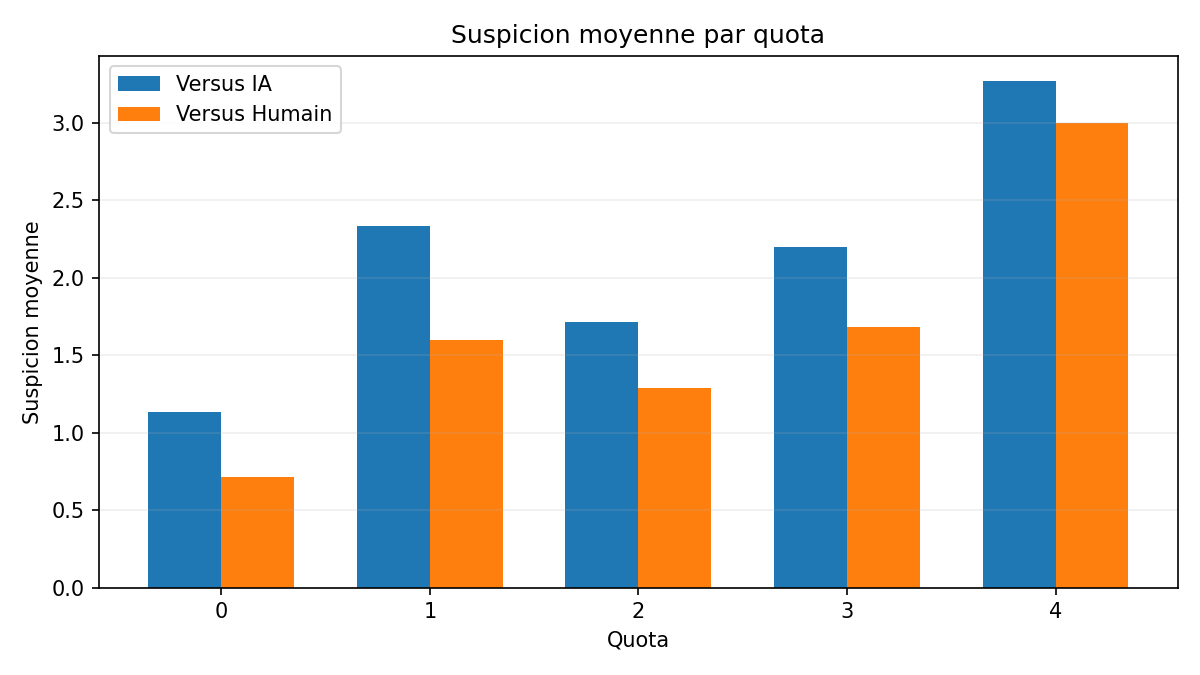
\includegraphics[width=0.85\textwidth]{../rapport/diagrams/plot_quota_comparison.png}
\end{center}
\end{frame}

\begin{frame}
\frametitle{Implications attendues}
\textbf{Si H\textsubscript{1} est confirmée :}
\begin{itemize}
    \item Les utilisateurs appliquent des standards différents selon le label
    \item Biais systématique dans la perception de tromperie artificielle
    \item Implications pour le design éthique d'IA
\end{itemize}

\vspace{0.5cm}

\textbf{Si H\textsubscript{1} est réfutée :}
\begin{itemize}
    \item La perception de déloyauté est basée sur le comportement, pas le label
    \item Questions sur la nature du biais anthropomorphe
\end{itemize}

\vspace{0.5cm}

\textbf{Résultats secondaires :}
\begin{itemize}
    \item Profils individuels de sensibilité à la triche
    \item Rôle de l'expérience préalable avec l'IA
    \item \todo{[Analyses explorathoires à définir]}
\end{itemize}
\end{frame}

% ═════════════════════════════════════════════════════════════════════════
% SECTION 6 : CONCLUSION
% ═════════════════════════════════════════════════════════════════════════

\section{Conclusion}

\begin{frame}
\frametitle{Contribution et avancées}
\textbf{Apports scientifiques :}
\begin{itemize}
    \item \textbf{Théorique} : Éclairage sur les mécanismes de confiance asymétrique
    \item \textbf{Méthodologique} : Protocole reproductible et rigoureux
    \item \textbf{Applicatif} : Recommandations pour design d'IA responsable
\end{itemize}

\vspace{0.5cm}

\textbf{Particularités du projet :}
\begin{itemize}
    \item Architecture web+Python flexible et scalable
    \item Contrôle expérimental absolu du comportement adversaire
    \item Collecte de données centralisée
    \item Intégrabilité future avec robot physique
\end{itemize}
\end{frame}

\begin{frame}
\frametitle{Perspectives futures}
\begin{itemize}
    \item \textbf{Extension} : Réintégration du robot Pepper (bottleneck résolu)
    \item \textbf{Variations} : Différents contextes compétitifs (poker, jeux de données)
    \item \textbf{Longitudinal} : Suivi de la confiance chez mêmes participants
    \item \textbf{Démographique} : Étude des facteurs individuels modulant le biais
\end{itemize}
\end{frame}

\begin{frame}
\frametitle{Merci}
\begin{center}
{\Large Pepper Battleship}

\vspace{1cm}

\textit{Détection de triche et confiance homme-machine}

\vspace{2cm}

\todo{Université - Master 1 Génie Logiciel}

\vspace{1cm}

Questions ?
\end{center}
\end{frame}

\end{document}
